\documentclass{article}
\usepackage[a4paper]{geometry}

\geometry{a4paper, total={170mm,257mm} ,left=20mm ,right=20mm ,top=20mm}
\usepackage{enumitem}
\usepackage{array}
\usepackage{tikz}
\usepackage{listings}
\usepackage{amsmath}
\usepackage{longtable}
\usepackage{multirow}
\usepackage{pgfplots}
\usepackage{minted}[cache=false]
\usepackage{subfig}
\usepackage{csvsimple}
\usepackage[english]{babel}
\usepackage[utf8]{inputenc}
\usepackage{fancyhdr}
\usepackage[hidelinks]{hyperref}
\usepackage{scrextend}

\pagestyle{fancy}
\fancyhf{}
\rhead{\large \rightmark}
\lhead{\large Machine Learning Investigation}
\rfoot{\large Page \thepage}
\lfoot{\large Name: Eris Brabham\\ Candidate Number: }

\newcounter{magicrownumbers}
\newcommand\rn{\stepcounter{magicrownumbers}\arabic{magicrownumbers}}
\newcommand\nrn{\stepcounter{magicrownumbers}\arabic{magicrownumbers}}
\usetikzlibrary{matrix,shapes,arrows,positioning,chains}

\newcolumntype{C}[1]{>{\centering\let\newline\\\arraybackslash\hspace{0pt}}m{#1}}
\newcolumntype{L}[1]{>{\raggedright\let\newline\\\arraybackslash\hspace{0pt}}m{#1}}
\newcolumntype{M}[1]{>{\centering\arraybackslash}m{#1}}
\newcolumntype{N}{@{}m{0pt}@{}}

\newcommand{\pluseq}{\mathrel{+}=}
\newcommand{\greatereq}{\mathrel{>}=}
\newcommand{\lesseq}{\mathrel{<}=}
\newcommand{\minitab}[2][l]{\begin{tabular}{#1}#2\end{tabular}}

\newminted[pythoncode]{python}{frame=leftline,framesep=2mm,baselinestretch=1.2,fontsize=\footnotesize,linenos}
\newminted[pseudocode]{markdown}{escapeinside=||,mathescape=true,frame=leftline,linenos,fontsize=\normalsize}

\def\mathLarge#1{\mbox{\huge $#1$}}

\tikzset{block/.style={rectangle,draw,text width=10em,text badly centered,rounded corners}}

\begin{document}

\begin{titlepage}
    \begin{center}
        \vspace*{3cm}
        {\Huge \textbf{An Investigation into Machine Learning and Neural Networks through the Simulation of Human Survival}} \\
        \vspace{1cm}
        {\Large Computer Science NEA}
        
        \vfill
        
        \large
        \textbf{Name:} Eris Brabham \\
        \textbf{Candidate Number:} \\
        \vspace{0.2cm}
        \textbf{Centre Name:} Barton Peveril College\\
        \textbf{Centre Number:} 58231\\
        \pagebreak
    \end{center}
\end{titlepage}

\large

\setcounter{tocdepth}{5}
\tableofcontents

\begin{flushleft}
    \section{Analysis}
        \subsection{Statement of Investigation}
            \large
            \vspace{0.2cm}
            I plan to investigate Machine Learning and Neural Networks by developing a Survival Simulation environment 
            in which a character will be controlled by a Machine Learning algorithm. \\
            \vspace{0.2cm}
            The Machine Learning Algorithm I choose to implement will most likely require lots of Complex Maths, from prior knowledge
            I know that Matrices and Calculus are heavily used within Neural Networks. Most of this Maths I will have 
            covered in my Maths and Further Maths Lessons, but some will require independant research on my Part. \\
            \vspace{0.2cm}
            The survival simulation will be procedurally generated and present multiple challenges 
            towards this character in order to provide a complex problem for it to solve. The procedural generation will
            be based upon a seed, and will generate Terrain which the character has to explore and navigate. The challenges 
            could be things like collecting items, or having to avoid/kill enemies which are actively tracking the character 
            and trying to hinder it's progress. \\
            \vspace{0.2cm}
            The key question I aim to answer with this investigation is:

            \begin{center}
                \vspace{0.3cm}
                \textbf{Can I develop a Machine Learning Algorithm to survive in a pseudorandom, open-world environment?}
                \vspace{0.3cm}
            \end{center}

            This question is rather broad and allows me to experiment with varying levels of complexity when it comes to
            the simulation. As long as I can implement a Machine Learning Algorithm which is complex enough to solve the 
            provided challenges. \\
            \vspace{0.2cm}
        \subsection{Background}
            \vspace{0.2cm}
            I am investigating Machine Learning because I've been wanting to try my hand at it for a while, this Project
            will allow me to gain a broad understanding of Neural Networks and their applications, along with an understanding
            of procedural generation. Machine Learning is an evolving field, with mere infinite applications from Image Recognition
            to Self Driving Cars. \\
            \vspace{0.2cm}
            \textbf{Old} \\ 
            I am investigating this area of Computer Science because I've been interesting in attempting a form of
            Machine Learning for a while now but havent had a reason to dive into it. Machine Learning is an evolving
            field, with mere infinite applications such as Image Recognition, Chat Bots, Self Driving Cars, 
            etc. I feel as though my project will be sufficiently advanced enough to expand my knowledge of the subject.
            It will require lots of research, planning, and design work in order to successfully fulfil my Technical
            Solution. \\

            \vspace{0.2cm}
        \subsection{Expert}
            \vspace{0.2cm}
            For my expert I approached one of my friends, Shaun, who has prior experience with Machine Learning. He has
            created his own Hand Written Digit Recognition Network before, along with using Python Libraries such as 
            \textit{PyTorch} to train an agent to play the game \textit{Flappy Bird}, among other ML projects. He has 
            a much better understanding of Machine Learning than me currently, so hopefully he will be a good resource 
            as I develop my project. \\

            \vspace{0.2cm}        
        \subsection{Initial Research}
            \subsubsection{First Interview}
                \large
                \vspace{0.2cm}
                As part of my Investigation I approached my friend Shaun, who has Experience with Machine Learning.
                I formed a list of questions to ask him, the responses are paraphrased for clarity. I mainly wanted to gain an idea of 
                what Machine Learning algorithm would suit my project the best. So I targetted my questions towards this. \\
                \vspace{0.2cm}
                \begin{enumerate}
                    \item {\large What are your first impressions of my project?} \\
                    \vspace{0.2cm}
                    “Your project is definitely very complex and if finished will tick alot of the boxes needed for Full Marks. There are lots
                    of layers of complexity along with room for good Object Orientated Design.”

                    \vspace{0.5cm}
                    \item {\large What Machine Learning Algorithms do you think would be relevant to my project?} \\
                    \vspace{0.2cm}
                    "Without pushing your complexity too far I think you should look into Deep Reinforcement Learning, I believe it has the
                    possibility of solving your problem if not too complex. Because of that you may way want to keep your simulation as minimal
                    as possible in order to give your Agent a chance. If you wanted to go further you could implement a Convolutional Neural Network, 
                    but this will add to the Complexity and take more time to program."

                    \vspace{0.5cm}
                    \item {\large Would User Defined Parameters be helpful?} \\
                    \vspace{0.2cm}
                    "The ability to dynamically change the parameters through a json file or similar would be very useful. Epecially to users who
                    have little to no experience with it before hand. The ability to change things like the Procedural Generation, Enemy Counts, 
                    Network Structure etc would be the perfect addition to your project."

                    \vspace{0.5cm}
                    \item {\large What Procedural Generation method would be best for my Project?} \\
                    \vspace{0.2cm}
                    "I only have experience with Perlin Noise but I think that it would be a great fit for your Project. It uses simple vector Maths
                    to calculate Gradient Noise, and is relatively simple to understand and Program. There are other Procedural Generation Methods
                    I'm aware of like Diamond Square or Simplex Noise, but both of those are much more complicated to my understanding."

                    \vspace{0.5cm}
                    \item {\large How complex should I make my Simulation?} \\
                    \vspace{0.2cm}
                    "I would stick to a relatively simple simulation at first, and then if your agent is successful at solving it, you can add more
                    to test the limits of your network after. Dynamic threats like Enemies which follow the Agent which it can attack would provide a base 
                    complex problem to start off with. Other problems could be collecting items or a simple Food Collection system with a Hunger Meter."

                    \vspace{0.5cm}
                    \item {\large How should I determine if my project is successful?} \\
                    \vspace{0.2cm}
                    "You could log a graph of Loss compared to Time, and in theory if your agent is learning it will successfully reduce the average Loss 
                    the more training it receives. You could use this graphed data as supporting evidence in your Evaluation."

                    \vspace{0.5cm}
                    \item {\large What should I focus my Initial Research on?} \\
                    \vspace{0.2cm}
                    "It would be benefical to you to research the Maths behind Neural Networks, specifically for Forward Propagation
                    and Back Propagation. The Maths behind it can get very complicated, along with being very hard to debug if a small error is made.
                    They both heavily rely on Matrix Operations, so if you're not familiar with those you should get up to speed."

                    \vspace{0.5cm}
                \end{enumerate}
                \subsubsection{Existing Investigations} 
                    \paragraph{Crafter} \mbox{} \\
                        \vspace{0.2cm}
                            In my research on the Internet I discovered a project called \textit{Crafter}. \\

                            \vspace{0.2cm}
                            \centerline{\textit{https://github.com/danijar/crafter}}
                            \vspace{0.2cm}

                            Crafter is described to be \textit{"Benchmarking the Spectrum of Agent Capabilities"}, and is utlised
                            in conjunction with Machine Learning Algorithms such as \textit{DreamerV2}, \textit{PPO} and \textit{Rainbow}. Crafter poses significant
                            challenge towards its Player, requiring high levels of generalisation, long-term reasoning, and complex 
                            problem solving. If the Machine Learning algorithm in question fails to achieve one of these aspects it will 
                            struggle to full "Solve" the simulation. \\

                            \vspace{0.2cm}

                            High levels of generalisation are required when training a Machine Learning algorithm, if this is not achieved then
                            your network will only lend itself to a single Dataset/Problem. An example of this would be training a network used
                            to recognise hand written digits on only one way of writing 4's, if presented with an input for a different type of 
                            4 it may not recognise it and identify it incorrectly. \\
                            
                            \vspace{0.2cm}

                            Long-Term reasoning is a complex problem to solve in the context of Machine Learning, current Machine Learning models
                            struggle to deal with this problem. This is dealt with by using algorithms built to mimic "memory". A common 
                            implementation of this is Experience Replay which stores states in a queue, and relearns from it after every N ammount
                            of steps. \\

                            \vspace{0.2cm}

                            A complex reward and action system may take time for an algorithm to learn but it certainly is possible with current
                            Machine Learning Models. Crafter utilises a complex action system with a flow chart determining which Action can be taken
                            given the current state of the simulation. Below is shown the Complex Flow Chart of Actions: \\

                            \vspace{0.2cm}
                            \begin{center}
                                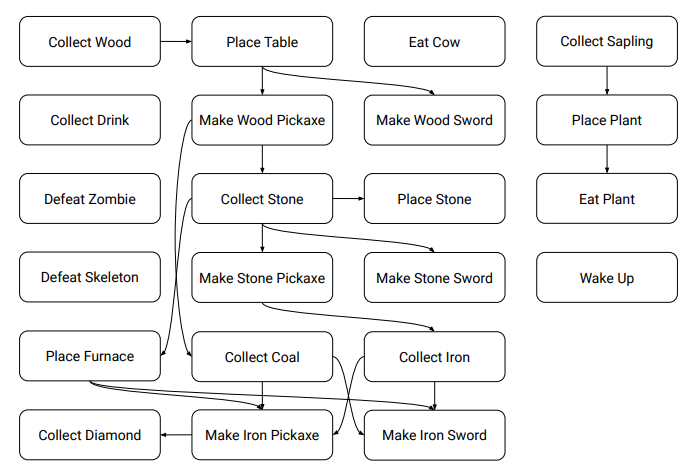
\includegraphics[width=12cm]{Images/InitialResearch/CrafterComplexActionSystem.PNG} \\
                                Complex action system as shown in the Paper "Benchmarking the Spectrum of Agent Capabilities" \\
                            \end{center}
                            \vspace{0.2cm}

                            Crafter manages to achieve quite high success rates with various Algorithms, but they still fail to overcome, or even match
                            human standards. This is likely due to the complexity of the problem, and in theory will be solvable within the near future
                            as Machine Learning advances over the next few years. This is why I plan to create a simpler simulation which the Agent will
                            be more likely to be able to solve. Below is shown the Success Rate Data for both Algorithms and Human Experts. \\

                            \begin{figure}[h]
                                \centering
                                \subfloat[\centering Success Rate of Algorithms]{{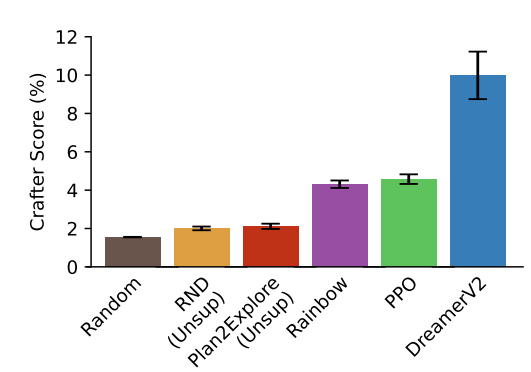
\includegraphics[width=7cm]{Images/InitialResearch/CrafterMLTrainingData.PNG}}}
                                \qquad
                                \subfloat[\centering Comparison Against Human Data]{{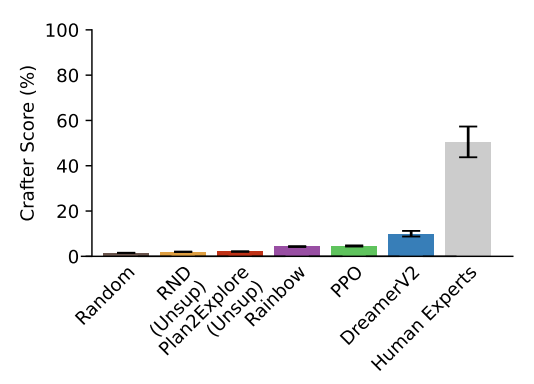
\includegraphics[width=7cm]{Images/InitialResearch/CrafterMLTrainingData+Human.PNG}}}
                            \end{figure}

                            While I would love to create a simulation similar to crafter, it is very complex and would take a long time to develop. Yet
                            would not net many marks in the process. Overall I feel like Crafter is a good example that my project is possible, but will
                            require a complex Machine Learning Model in order to achieve reliable results from my Investigation.

                    \paragraph{Minecraft} \mbox{} \\
                        \vspace{0.2cm}
                        Minecraft is a \textit{very} popular Game. It's a sandbox game, meaning that the player can do almost anything they want.
                        The game is formed from blocks which can be broken or placed, along with a plethera of items, enemies, passive animals
                        and more. It has infinite terrain generation, and explicity uses Perlin Noise. The seed of the noise determines
                        all the terrain generation, loot tables, random structures, caves, etc. \\
                        
                        \vspace{0.2cm}

                        First it starts off on a very broad level, painting a basic topographical map of the world. It uses Perlin Noise to sample
                        a height value for each chunk, where chunks are 16x16 areas of blocks. Then within these chunks the game uses the Diamond Square
                        algorithm to interpolate between it and the chunks around it, creating blocks where the terrain should be. This produces an 
                        entirely deterministic results based upon the seed.\\

                        \vspace{0.2cm}

                        Secondly, the Caves are generated using Perlin Worms, which travel in deterministic directions based on their starting position.
                        These worms dig through the terrain carving out caves which can then be traversed by the player. Within these Caves spawn water
                        sources, pools of lava, useful ores. All of these are deterministically generated by the original seed. \\ 


                        \begin{figure}[h]
                            \centering
                            \subfloat[\centering Example of Minecraft's terrain generation in a Swamp Biome]{{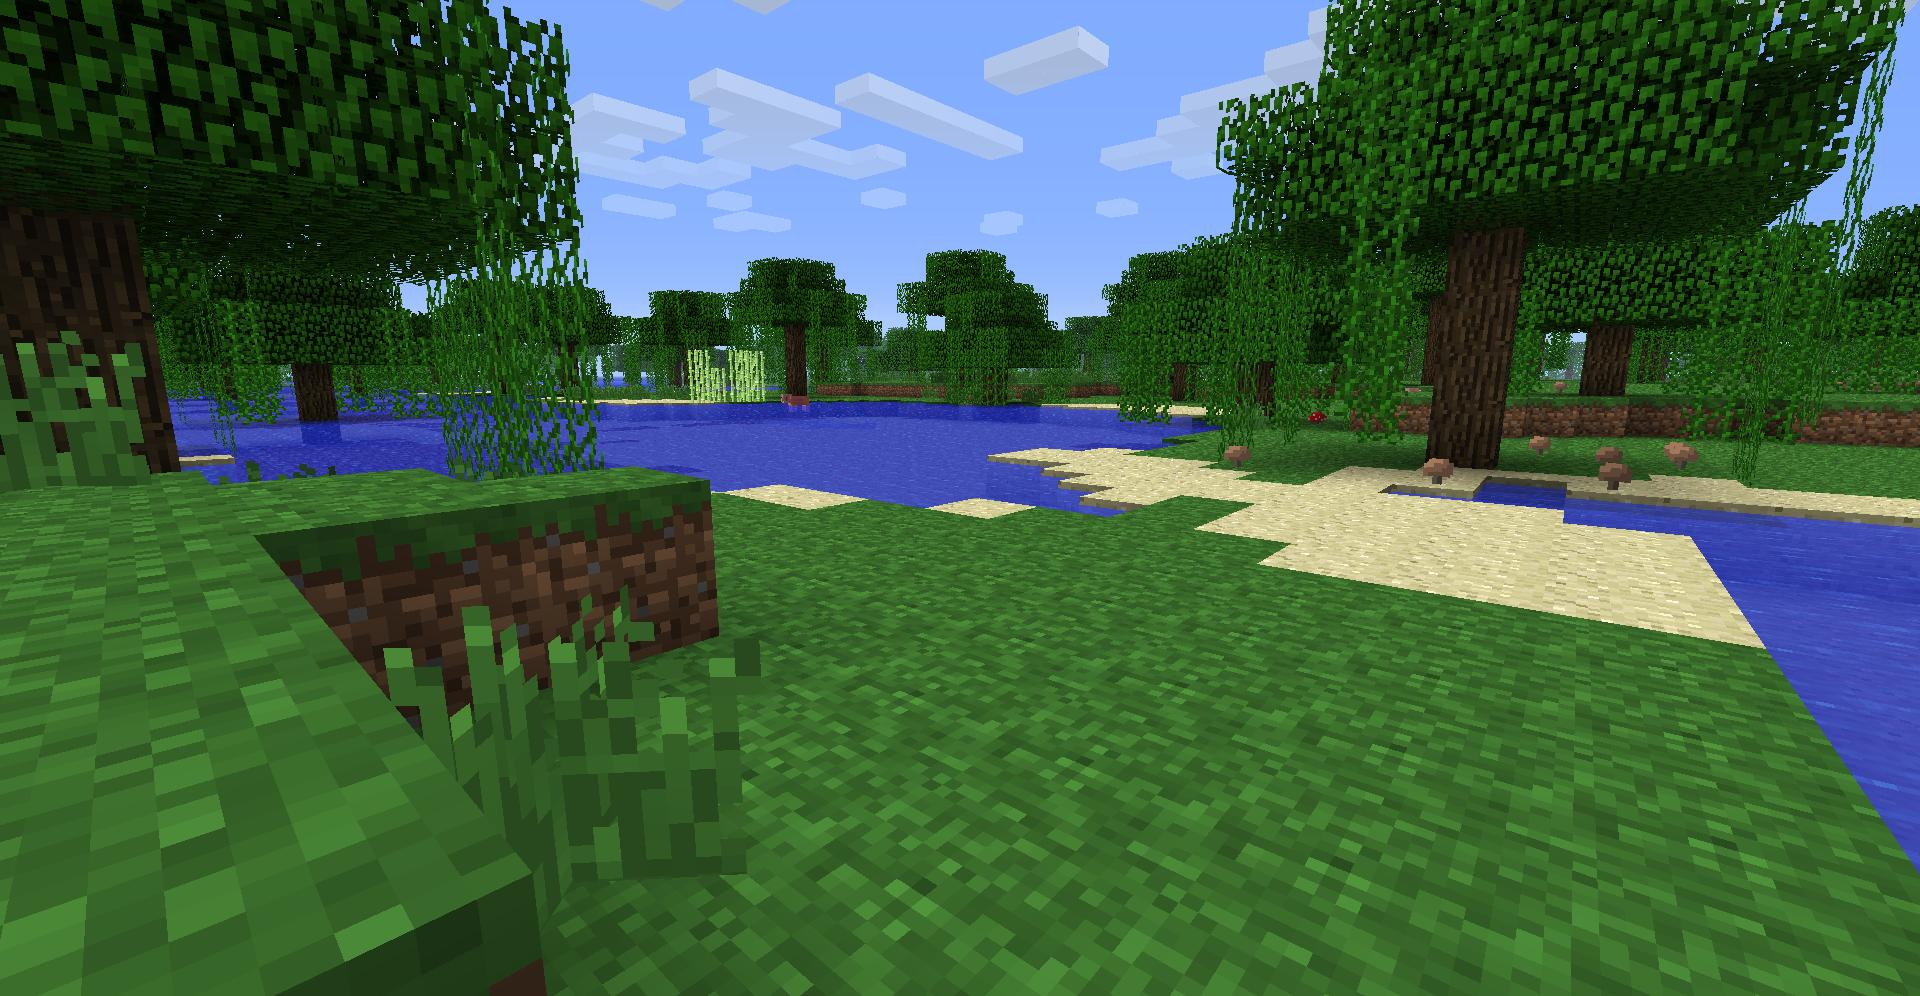
\includegraphics[width=8cm]{Images/InitialResearch/MCTerrainGeneration.jpg}}}
                            \qquad
                            \subfloat[\centering Example of a Sunken Pirate Ship Structure]{{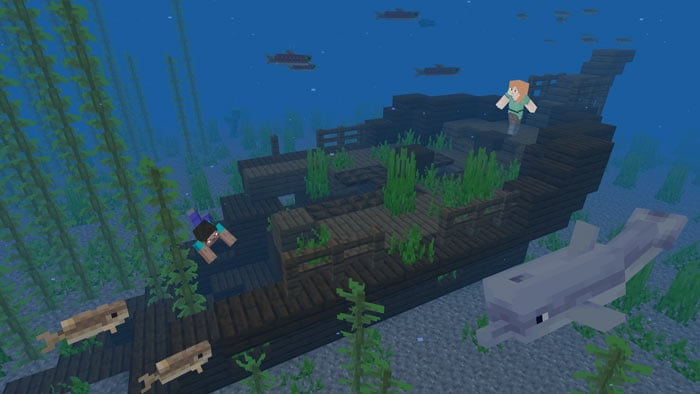
\includegraphics[width=8cm]{Images/InitialResearch/MCStructureGeneration.jpg}}}
                        \end{figure}

                        Minecraft itself is too complex and dynamic to be solved by current Machine Learning algorithms, along with there is no quantifiable 
                        metric for performance due to it's sandbox nature. There exist data sets for Minecraft, in the form of captured gameplay footage, but
                        there has been little to no success of quantifiably good solutions to solving Machine Learning problems within Minecraft. \\

                        \vspace{0.2cm}

                        Overall I feel like it would be good to borrow elements from Minecraft's terrain generation, such as its utilisation of Perlin Noise.
                        But the majority of the games systems are way too complex for a Machine Learning algorithm to solve. \\

                    \paragraph{Conway's Game of Life} \mbox{} \\
                        \vspace{0.2cm}
                        Conway's Game of Life is whats called a Cellular Automaton, which is a discrete computation model formed from a grid of cells along with 
                        a ruleset. Conway's is commonly referred to a Zero Player Game, where the input for the Automaton is defined at the start, with no
                        further adjustment needed for it to run. The game is fully Turing complete and can simulate a Universal Constructor. \\
                        \vspace{0.2cm}
                        The rules of Conway's are such that: \\

                        \vspace{0.2cm}
                        \begin{addmargin}[2em]{0em}
                            \large
                            1. Any live cell with fewer than two live neighbours dies, as if by underpopulation. \\
                            2. Any live cell with two or three live neighbours lives on to the next generation. \\
                            3. Any live cell with more than three live neighbours dies, as if by overpopulation. \\
                            4. Any dead cell with exactly three live neighbours becomes a live cell. \\
                        \end{addmargin}

                        \vspace{0.2cm}
                        It is rather interesting that such complicated Machines can be formed from such a simple ruleset, as an example 
                        here is a Turing Machine formed from 34 Thousand Cells: \\

                        \begin{figure}[h]
                            \centering
                            \subfloat[\centering Turing Machine built in Conways Game of Life]{
                                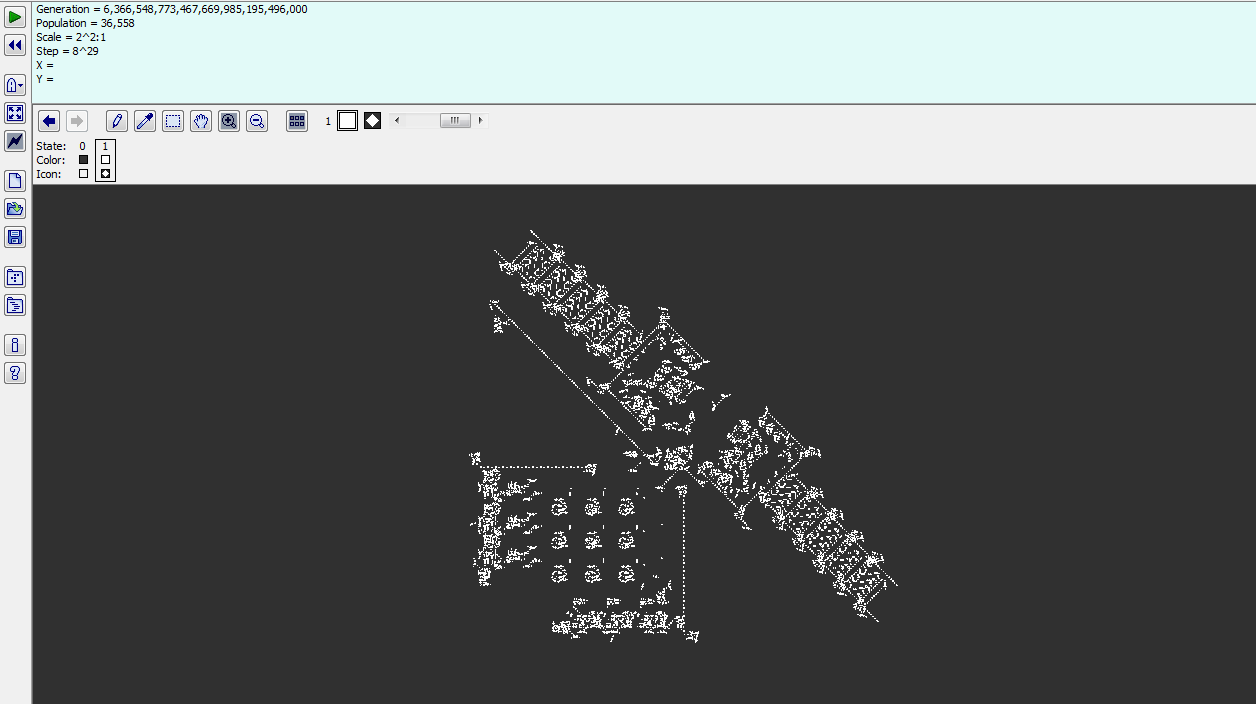
\includegraphics[width=14cm]{Images/InitialResearch/ConwaysTuringMachine.png}}
                        \end{figure}

                        Overall, I think this shows that my simulation doesnt need to have complex rules in order to achieve 
                        interesting results. Conway's is formed from 4 simple rules, and yet is Turing complete.

                \subsubsection{Algorithms and Potential Data Types}
                    \large
                    \vspace{0.2cm}
                    \paragraph{Neural Network and Matrices} \mbox{} \\
                        As part of developing a Machine Learning Algorithm, I will need to implement a Matrix class in order to
                        implement a Neural Network. Matrices are commonly used to represent individual layers of a network. Along
                        with making calculations much easier, condensing them into performing operations on matrices, rather than
                        using nested for loops and lists. As part of my Initial Research I have taken the time to understand
                        how a Neural Network functions, it turns out I have already learned most of the Maths needed to understand
                        how it works in my A Level Maths and Further Maths courses. \\
                        \vspace{0.2cm}
                        A Neural Network functions as a series mathematical equations used to recognise relationships between inputs
                        and desired outputs. They take in a Vector of Input Data, and output a Vector of Output Data. They can be represented
                        in simple terms as a function: $N(x)$ where: $\{x \in V, N(x) \in V\}$, should you adopt the black box approach. 
                        The functions name in this case is Forward Propagation. \\
                        \vspace{0.2cm}
                        We form a Neural Network with multiple layers of Nodes, the layers being referred to as the Input Layer, 
                        Hidden Layer/s and Output Layer. In this case each Node is connected to every Node in the previous layer and
                        the following layer. In the below image is represented a Neural Network with a layer structure of $[3, 5, 2]$.

                        \vspace{0.1cm}
                        \centerline{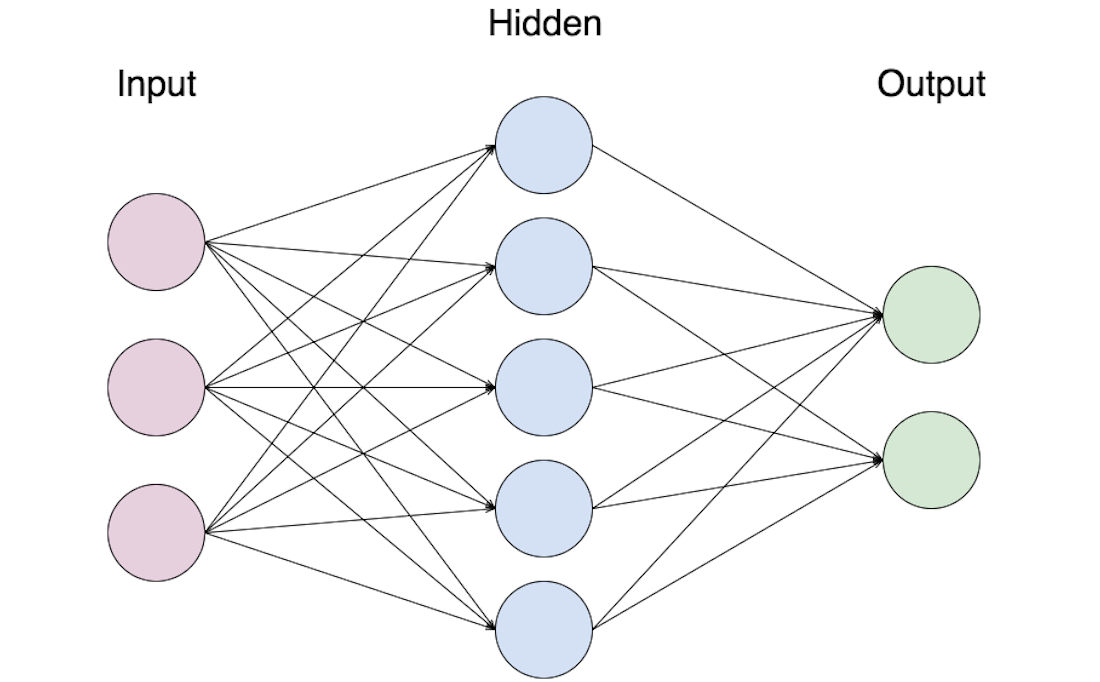
\includegraphics[width=10cm]{Images/InitialResearch/NeuralNetworkExample.png}}

                        Each connection, otherwise known as an Arc or Edge, has an associated weight. Along with every output of a
                        layer having an associated Bias. These are used to compute the outcome of a network. \\
                        \vspace{0.2cm}
                        Forward Propagation is used to compute the outcome of a network, it has a general form and uses 
                        Matrix Multiplication and Addition to achieve this.
                        \vspace{0.2cm}
                        
                        \begin{center}
                            $
                            S^{(L)} = 
                            \begin{bmatrix}
                            s^{(L)}_{0} \\
                            s^{(L)}_{1} \\
                            \vdots      \\
                            s^{(L)}_{n} 
                            \end{bmatrix}
                            = 
                            \begin{bmatrix}
                            w^{(L-1)}_{0,0} & w^{(L-1)}_{0,1} & \hdots  & w^{(L-1)}_{0,m} \\
                            w^{(L-1)}_{1,0} & w^{(L-1)}_{1,1} & \hdots  & w^{(L-1)}_{1,m} \\
                            \vdots          & \vdots          & \ddots  & \vdots          \\
                            w^{(L-1)}_{n,0} & w^{(L-1)}_{n,1} & \hdots  & w^{(L-1)}_{n,m} \\
                            \end{bmatrix}
                            \begin{bmatrix}
                            a^{(L-1)}_{0} \\
                            a^{(L-1)}_{1} \\
                            \vdots      \\
                            a^{(L-1)}_{n} 
                            \end{bmatrix}
                            +
                            \begin{bmatrix}
                            b^{(L)}_{0} \\
                            b^{(L)}_{1} \\
                            \vdots      \\
                            b^{(L)}_{n} 
                            \end{bmatrix}
                            $ 
                        \end{center}
                        
                        \begin{center}
                            $
                            \sigma(S^{(L)})
                            =
                            \sigma\left(
                            \begin{bmatrix}
                            s^{(L)}_{0} \\
                            s^{(L)}_{1} \\
                            \vdots      \\
                            s^{(L)}_{n} 
                            \end{bmatrix}
                            \right)
                            =
                            \begin{bmatrix}
                            \sigma(s^{(L)}_{0}) \\
                            \sigma(s^{(L)}_{1}) \\
                            \vdots              \\
                            \sigma(s^{(L)}_{n}) 
                            \end{bmatrix}
                            $ 
                        \end{center}
                        
                        \vspace{0.2cm}
                        We then apply an activation function as shown above, in this case we will apply the Sigmoid function: $\sigma(x)$ to $S^{(L)}$. 
                        The Sigmoid function is a Mathematical Function which \textit{squishes} values between 0 and 1. Shown Below:
                        
                        \begin{center}
                            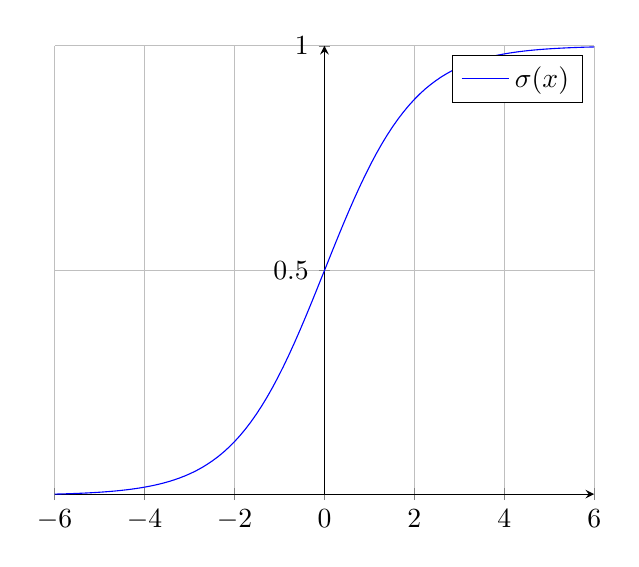
\begin{tikzpicture}[declare function={sigma(\x)=1/(1+exp(-\x));}]
                            \begin{axis}%
                            [
                                grid=major,     
                                axis x line=bottom,
                                ytick={0,.5,1},
                                ymax=1,
                                axis y line=middle,
                                samples=100,
                                domain=-6:6,
                                range=0:1
                                legend style={at={(1,0.9)}}     
                            ]
                                \addplot[blue,mark=none]   (x,{sigma(x)});
                                \legend{$\sigma(x)$}
                            \end{axis}
                            \end{tikzpicture}
                        \end{center}

                        Matrices can be used for all parts of a Neural Network implementation, and will prove very useful in my Technical
                        Solution. \\

                    \paragraph{Procedural Generation} \mbox{} \\
                        \vspace{0.2cm}
                        For my project I am going to have to procedurally generate 2d terrain, while researching this I came across a few algorithms
                        which seemed to be able to do this pretty well. I will compare two algorithms I discovered below.
                        
                        \begin{center}
                            \begin{tabular}{| L{6cm} | L{6cm} |}
                                \hline
                                {\large Post-Processing Algorithms} & {\large Perlin Noise} \\
                                \hline
                                I discovered two post processing algorithms often used for simple 2d terrain generation. 1 Averages squares 
                                around the selected square, and the other pulls it up or down the gradient its currently on.
                                I find these interesting because they're relatively simple, and I'm not quite sure whether they will produce good results or not. 
                                So it would be interesting to test out implementing these in my prototype.
                                &
                                Perlin Noise is an algorithm developed by Ken Perlin for use in the digital generation of noise.
                                This noise can be combined to create \textit{realistic} looking height maps for world generation.
                                Perlin Noise retains continuity and is seeded so the generation can be entirely controlled.
                                By "retains continuity" I mean that you can sample the same point and retrieve the same value. 
                                If I was to implement Perlin noise it would take longer, but also might end up with a better result
                                due to it being more widely used. It's a trade-off between time to implement and desired result. \\
                                \hline
                            \end{tabular}
                        \end{center}
                        
                        I also discovered an algorithm called Poisson Disc Sampling, this can be used to sample random points 
                        in N dimensional space. It takes in 2 values, the R and K value, these values determine the output of
                        the function. The R values is the minimum distance a point has to be from another, randomly placed point
                        which hasn't been selected yet. If the distance between any existing points is less than R, the point
                        will be rejected and another will be selected. The K value determines how many rejected are needed before 
                        the algorithm will stop attempting to choose a new point.
                        
                    \paragraph{Proposed Programming Language and Associated Libraries} \mbox{} \\
                        \vspace{0.2cm}
                        When selecting a Programming Language and associated Graphical Libraries I took into consideration a few options.
                        Below I have weighed up 3 options for Programming Language, along with 2 graphical libraries per language
                        
                        \begin{center}
                            \begin{tabular}{|M{2cm}|M{2cm}|M{8cm}|}
                                \hline
                                    Proposed Solution & \multicolumn{2}{M{10cm}|}{Benefits and Downsides of Proposed Solution} \\
                                \hline
                                    Python & \multicolumn{2}{M{10cm}|}{Python is the first thought which comes to mind when I think about programming, 
                                    it is my favourite language and I'm yet to find anything which I prefer. Its very versatile and great
                                    for rapid prototyping, the dynamic typing makes It great for coding quickly without worrying too
                                    much about whether you're using a \textit{float32 or float64}. It also has hundreds of libraries
                                    and is very well supported by its developers and the community.}\\
                                \hline
                                    \multirow{2}*{\minitab[c]{Python \\ Graphical \\ Libraries}} & Pygame & Pygame is a highly customizable and well developed binding of
                                    \textit{Simple DirectMedia Layer} (SDL) Library. It has a full set of 2d drawing tools, along with keyboard and audio
                                    capabilities. I have lots of experience with Pygame so I already have code which I can take from, which will speed up
                                    development when dealing with the Pygame library.\\
                                \cline{3-3}
                                    &Tkinter & Tkinter provides an interface to the standard \textit{Tcl/Tk GUI Toolkit}, which is available
                                    for most platforms, this makes it highly versatile. Though as my project is not intended as a software
                                    package I dont see this as being an incredibly big selling point. Tkinter will serve mostly the same
                                    purpose as Pygame but give me easier options for Graphical Input, I dont currently plan to add GUI so 
                                    this feature isnt neccesary.\\
                                \hline
                            \end{tabular}

                            \begin{tabular}{|M{2cm}|M{2cm}|M{8cm}|}
                                \hline
                                    Proposed Solution & \multicolumn{2}{M{10cm}|}{Benefits and Downsides of Proposed Solution} \\
                                \hline
                                    C\# & \multicolumn{2}{M{10cm}|}{C\# is my second favourite language, I have plenty of experience with it from developing games
                                    with Unity. It's faster than Python and is less abstracted, but this speed isn't necessarily required
                                    for my project. With C\# I could utilise the \textit{Unity Game Engine} for my project, but then
                                    I might end-up relying on builtin types and functions rather than developing my own.}\\
                                \hline
                                    \multirow{2}*{\minitab[c]{C\# \\ Graphical \\ Libraries}} & Windows Forms & Windows Forms is a relatively simple drag drop
                                    interface for designing your own applications. I've never used it before but I could utilise it with C\# to create my project.
                                    I belive it might be a bit overkill for my needs though, as it includes many, many UI features which I will have no use for.\\
                                \cline{3-3}
                                    & WPF & WPF or \textit{Windows Presentation Foundation} is a versatile development platform for desktop applications.
                                    It is relatively versatile in its uses and utilises XAML and is the UI Language of Windows Platforms. XAML would be a
                                    new language for me to learn but I have experience with HTML so I dont believe it would be too difficult.
                                    The platform would provide a stable base to my project.\\
                                \hline
                            \end{tabular}

                            \begin{tabular}{|M{2cm}|M{2cm}|M{8cm}|}
                                \hline
                                    Proposed Solution & \multicolumn{2}{M{10cm}|}{Benefits and Downsides of Proposed Solution} \\
                                \hline
                                    Rust & \multicolumn{2}{M{10cm}|}{Rust is low level language designed for speed and efficiency, I started using it recently
                                    as a side hobby and would like to use it more in future projects of mine. Though I feel like it may be a bit overkill for a Computer 
                                    Science NEA, with it often being used for server side applications rather than general purpose applications.}\\
                                \hline
                                    \multirow{2}*{\minitab[c]{Rust \\ Graphical \\ Libraries}} & Piston2d & Piston2d is a feature complete 2d graphics library which utilises OpenGl,
                                    I've worked with it briefly before and I believe it would be a good option over Pixels if I needed more complex drawing
                                    methods.\\
                                \cline{3-3}
                                    & Pixels & Pixels is a lightweight 2d graphics library designed to simply push pixels to the screen, Its relatively simple
                                    and i've used it for making a simple \textit{Falling Sand Game} before, could be a good little option if I wanted to develop
                                    a lightweight solution.\\
                                \hline
                            \end{tabular}
                        \end{center}

        \subsection{Prototype}
            \subsubsection{Prototype Objectives}
            \large
            \vspace{0.2cm}
            Before starting my Prototype I had to decide upon a short list of objectives I wanted to 
            complete/investigate as part of it. These boiled down to a few things:

            \vspace{0.2cm}
            \begin{itemize}
                \item Terrain Generation
                \item Displaying the Generated Terrain using a Graphics Library
                \item Matrix and Vector implementation
            \end{itemize}
            \vspace{0.2cm}

            For my Prototype, I first created a GitHub Repository, available here: 
            
            \vspace{0.1cm}
            \centerline{\textit{https://github.com/TheTacBanana/CompSciNEAPrototype}}
            \vspace{0.1cm}

            I had created a hierarchy of importance for development in my head, visualized using this flow diagram:

            \begin{center}
                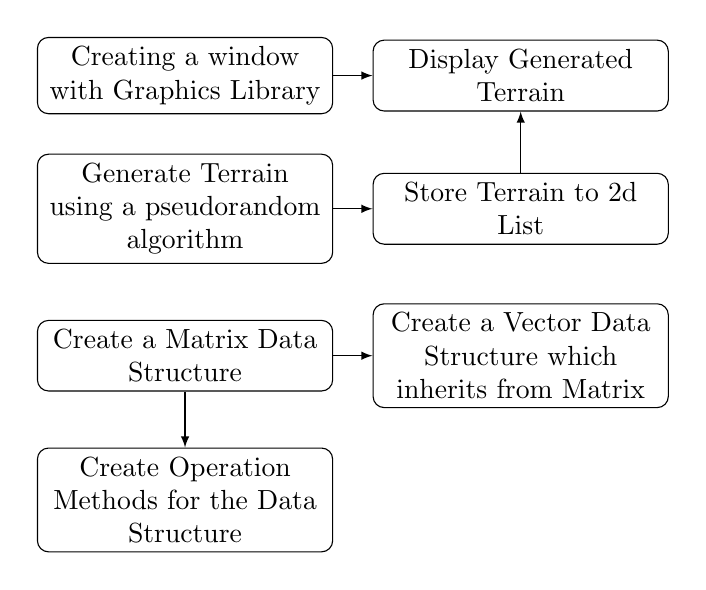
\begin{tikzpicture}
                    \matrix (m)[matrix of nodes, column  sep=0.5cm,row  sep=0.5cm, align=center, nodes={rectangle,draw, anchor=center} ]{
                        |[block]| Creating a window with Graphics Library &  |[block]| Display Generated Terrain \\   
                        |[block]| Generate Terrain using a pseudorandom algorithm &  |[block]| Store Terrain to 2d List \\
                        |[block]| Create a Matrix Data Structure & |[block]| Create a Vector Data Structure which inherits from Matrix \\
                        |[block]| Create Operation Methods for the Data Structure & \\
                    };
                    \path [>=latex,->] (m-1-1) edge (m-1-2);
                    \path [>=latex,<-] (m-1-2) edge (m-2-2);
                    \path [>=latex,->] (m-2-1) edge (m-2-2);
                    \path [>=latex,->] (m-3-1) edge (m-3-2);
                    \path [>=latex,->] (m-3-1) edge (m-4-1);
                \end{tikzpicture}
            \end{center}

            I decided to use Python for developing my Prototype, this seemed like a good fit due to me 
            having lots of experience with the language. Python is a Dynamically Typed and interpreted 
            which makes it versatile for protyping and fast, iterative development.
            
            \subsubsection{Terrain Generation and Displaying to Window}
            Starting from the begining of my hierarchy I installed Pygame using \textit{pip} and started creating a window.
            This was a relatively simple task only taking a few lines:
            \vspace{0.5cm}

            \normalsize
            \begin{pythoncode}
import pygame

simSize = 128
gridSize = 2

window = pygame.display.set_mode((simSize*gridSize, simSize*gridSize))
pygame.display.set_caption("Procedural Generation")

running = True
while running == True:
  for event in pygame.event.get():
    if event.type == pygame.QUIT:
      running = False
            \end{pythoncode}

            \vspace{0.5cm}

            \large
            This creates a window like this: \\ 
            \vspace{0.5cm}
            \centerline{
\includegraphics{Images/Prototype/CreateWindowExample.PNG}}

            \vspace{0.5cm}

            Following the hierarchy I then added noise generation by generating random numbers and 
            assigning them to a 2d List. Shown here: 
            
            \begin{pythoncode}
def GenerateMap(self, seed):
    random.seed(seed)
    for y in range(0, self.arraySize):
        for x in range(0, self.arraySize):
            self.heightArray[x][y] = round(random.random(),2)
        \end{pythoncode}

            \vspace{0.5cm}

            \large
            After creating some code to draw squares based upon the random value, I ended up with this 
            random array of Black-White squares:\\
            \vspace{0.5cm}
            \centerline{
\includegraphics{Images/Prototype/RandomNoiseExample.PNG}}

            \vspace{0.5cm}

            This was a good start, but didnt really look like terrain yet. As part of my research I came 
            across simple algorithms to turn random noise into usable 2d terrain. I decided to implement
            these algorithms. They are relatively short and didnt take too much time to implement. I've
            named the two algorithms UpDownNeutralGen and Average.

            \vspace{1cm}

            \paragraph{UpDownNeutralGen Method} \mbox{} \\
            \vspace{0.25cm}

            The UpDownNeutralGen method takes a tile, and considers every tile around it. It sums the tile 
            which are greater than, less than, or within a certain range of the tile height. And then pulls
            the selected tile in the direction which has the highest precedence. As an example, here are some
            randomly generated values:

            \begin{center}
                \begin{tabular}{| C{0.75cm} | C{0.75cm} | C{0.75cm} |}
                    \hline
                    0.71 & 0.19 & 0.3 \\ [0.75cm]
                    \hline
                    0.46 & 0.26 & 0.82 \\ [0.75cm]
                    \hline
                    0.63 & 0.35 & 0.05 \\ [0.75cm]
                    \hline
                \end{tabular}
            \end{center}

            If we count the surrounding values into corresponding Higher, Lower and Neutral we get: \\

            \begin{center}
                \begin{tabular}{| M{2cm} | M{2cm} | M{2cm} |}
                    \hline
                    Higher & Lower & Neutral \\ [0.25cm]
                    \hline
                    4 & 1 & 3 \\ [0.25cm]
                    \hline
                \end{tabular}
            \end{center}

            \vspace{0.5cm}

            This leads us to calculating the \textit{pullValue}, respectively for each case:
            \begin{eqnarray*}
                \text{pullValue } &=& 
                \begin{cases}
                    \text{upTiles} \times 0.09 & \text{Most Up Tiles} \\
                    \text{downTiles} \times -0.08 & \text{Most Down Tiles} \\
                    0 & \text{Most Neutral Tiles} 
                \end{cases} \\
                \text{Value}[x][y] &=& \text{pullValue}
            \end{eqnarray*}
            
            \vspace{0.5cm}

            We then add the pullValue to the original square value, leaving us with the updated value.
            The code for this is shown below:
            \begin{pythoncode}
def UpNeutralDownGen(self):
    dupMap = self.heightArray
    for y in range(0, self.arraySize):
        for x in range(0, self.arraySize):
            up = 0
            down = 0
            neutral = 0
            pointArr = []

            if x != 0 and y != 0:
                pointArr.append(self.heightArray[x - 1][y - 1])
            if x != 0 and y != self.arraySize - 1:
                pointArr.append(self.heightArray[x - 1][y + 1])
            if x != self.arraySize - 1 and y != self.arraySize - 1:
                pointArr.append(self.heightArray[x + 1][y + 1])
            if x != self.arraySize - 1 and y != 0:
                pointArr.append(self.heightArray[x + 1][y - 1])
            if x != 0:
                pointArr.append(self.heightArray[x - 1][y])
            if y != 0:
                pointArr.append(self.heightArray[x][y - 1])
            if x != self.arraySize - 1:
                pointArr.append(self.heightArray[x + 1][y])
            if y != self.arraySize - 1:
                pointArr.append(self.heightArray[x][y + 1])

            for i in range(len(pointArr)):
                if pointArr[i] >= self.heightArray[x][y] + 0.1:
                    up += 1
                elif pointArr[i] <= self.heightArray[x][y] - 0.1:
                    down += 1
                else:
                    neutral += 1

            if (up > down) and (up > neutral): # Up
                value = 0.09 * up
            elif (down > up) and (down > neutral): # Down
                value = -0.08 * down
            else: # Neutral
                value = 0

            dupMap[x][y] += value
            dupMap[x][y] = self.Clamp(dupMap[x][y], 0, 1)

    self.heightArray = dupMap
            \end{pythoncode}

            \paragraph{Average Method} \mbox{} \\
            \vspace{0.25cm}

            The Average method takes a tile and considers every tile around it, this time instead of looking at the
            differences, it creates an average from the 8 surrounding tiles. It then sets the selected tile to this
            average value. As an example, here are some randomly generated values:

            \begin{center}
                \begin{tabular}{| C{0.75cm} | C{0.75cm} | C{0.75cm} |}
                    \hline
                    0.83 & 0.93 & 0.64 \\ [0.75cm]
                    \hline
                    0.07 & 0.38 & 0.21 \\ [0.75cm]
                    \hline
                    0.33 & 0.94 & 0.95 \\ [0.75cm]
                    \hline
                \end{tabular}
                \vspace{0.25cm}

                Summing these and dividing by the total ammount of tiles grants us the average:

                \begin{eqnarray*}
                    \frac{0.83 + 0.93 + 0.64 + 0.07 + 0.38 + 0.21 + 0.95 + 0.33 + 0.94}{9} &=& 0.586 \\
                    Value[x][y] &=& 0.586
                \end{eqnarray*}
            \end{center}
            \vspace{0.25cm}

            The code for this is shown below:
            \begin{pythoncode}
def AverageGen(self):
    dupMap = self.heightArray
    for y in range(0, self.arraySize):
        for x in range(0, self.arraySize):        
            total = 0
            count = 0
            if x != 0 and y != 0:
                total += self.heightArray[x - 1][y - 1]
                count += 1
            if x != 0 and y != self.arraySize - 1:
                total += self.heightArray[x - 1][y + 1]
                count += 1
            if x != self.arraySize - 1 and y != self.arraySize - 1:
                total += self.heightArray[x + 1][y + 1]
                count += 1
            if x != self.arraySize - 1 and y != 0:
                total += self.heightArray[x + 1][y - 1]
                count += 1
            if x != 0:
                total += self.heightArray[x - 1][y]
                count += 1
            if y != 0:
                total += self.heightArray[x][y - 1]
                count += 1
            if x != self.arraySize - 1:
                total += self.heightArray[x + 1][y]
                count += 1
            if y != self.arraySize - 1:
                total += self.heightArray[x][y + 1]
                count += 1

            dupMap[x][y] = total / count
    self.heightArray = dupMap
            \end{pythoncode}

            \subsubsection{Finished Terrain Generation}
            \vspace{0.25cm}

            Overall I am happy with the Terrain generation, though I feel as if it could be improved to look more realistic.
            The difference between the original random noise and the Colour Mapped Terrain looks so much better.

            \begin{figure}[h]
                \centering
                \subfloat[\centering Grayscale Terrain Generation]{{
\includegraphics[width=6cm]{Images/Prototype/Seed420 Grayscale.png}}}
                \qquad
                \subfloat[\centering Colour Bands applied to the Terrain Generation]{{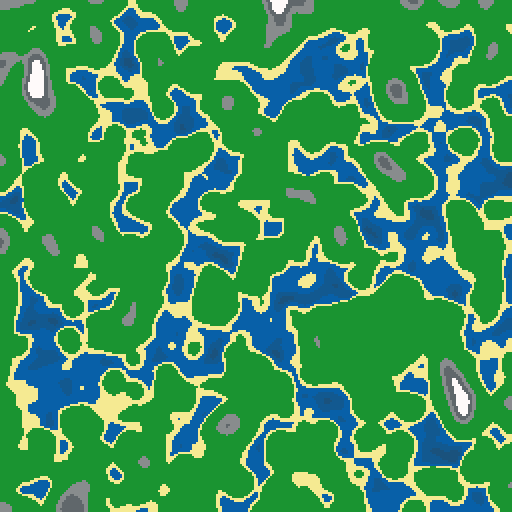
\includegraphics[width=6cm]{Images/Prototype/Seed420 Colour.png} }}
            \end{figure}
            
            \subsubsection{Matrix Data Structure}
                \vspace{0.25cm}

                As part of my Matrix Class I made a list of operations which would be key to a Matrix Class, along with being useful
                for Machine Learning. A Matrix is an abstract data type, commonly used in Maths, but has practical uses in the world
                of Computer Science. It holds a 2d array of values such as: \\ 
                \begin{center}
                $\begin{bmatrix}
                    a & b\\
                    c & d
                \end{bmatrix}$ 
                $\begin{bmatrix}
                    a & b & c \\
                    d & e & f \\
                    g & h & i 
                \end{bmatrix}$ 
                $\begin{bmatrix}
                    a \\
                    b \\
                    c  
                \end{bmatrix}$ 
                $\begin{bmatrix}
                    a & b & c & d\\
                    e & f & g & h
                \end{bmatrix}$ 
                \end{center}
                The values in a Matrix can be manipulated using common operations such as $+ - *$ as long as the orders of the 2 Matrices
                match up. Along with other, non-standard operations which have other purposes.

                \vspace{0.25cm}
                As part of my Matrix Class, I implemented the following operators:
                \begin{enumerate}
                    \item Addition/Subtraction \\
                        Implementing Addition didnt take too long, I utilised a nested for loop to iterate over every value in both Matrices.
                        Adding the two values together into a temporary Matrix which the method then returned. 
                        \vspace{0.25cm}
                        \begin{center}
                            $\begin{bmatrix}
                                a & b\\
                                c & d
                            \end{bmatrix} +
                            \begin{bmatrix}
                                e & f\\
                                g & h
                            \end{bmatrix} =
                            \begin{bmatrix}
                                a+e & b+f\\
                                c+g & d+h
                            \end{bmatrix}$
                        \end{center}
                        \vspace{0.25cm}

                        The written code is shown below:
                        \begin{pythoncode}
@staticmethod
def MatrixAddSubtract(m1, m2, subtract = False):
    m1Dims = m1.Dimensions()
    newMat = Matrix(m1Dims[0], m1Dims[1])
    for y in range(0, m1Dims[0]):
        for x in range(0, m1Dims[1]):
            if subtract:
                newMat.matrixArr[y][x] = m1.Val()[y][x] - m2.Val()[y][x]
            else:
                newMat.matrixArr[y][x] = m1.Val()[y][x] + m2.Val()[y][x]
    return newMat
                        \end{pythoncode}

                    \item Multiplication \\
                        Multiplication of Matrices is slightly more complicated, it is of $O(n^3)$ complexity, utilising a triple nested for loop.
                        It multiplies the row of a $M1$, by the column in $M2$. Summing the calculation into the element in the new Matrix $M3$. \\
                        
                        \vspace{0.25cm}
                        \begin{center}
                            $\begin{bmatrix}
                                a & b\\
                                c & d
                            \end{bmatrix} \times
                            \begin{bmatrix}
                                e & f\\
                                g & h
                            \end{bmatrix} =
                            \begin{bmatrix}
                                a*e + b*g & a*f + b*h\\
                                c*e + d*g & c*f + d*h
                            \end{bmatrix}$
                        \end{center}
                        There is also Scalar Multiplication which multiples each value of a Matrix by the Scalar.
                        \begin{center}
                            $k *
                            \begin{bmatrix}
                                a & b\\
                                c & d
                            \end{bmatrix} =
                            \begin{bmatrix}
                                ka & kb\\
                                kc & kd
                            \end{bmatrix}$
                        \end{center}
                        \vspace{0.25cm}

                        The written code is shown below:
                        \begin{pythoncode}
@staticmethod                        
def ScalarMultiply(s, m1):
    m1Dims = m1.Dimensions()
    newMat = Matrix(m1Dims[0], m2Dims[1])
    for y in range(0, m1Dims[0]):
        for x in range(0, m1Dims[1]):
            newMat.matrixArr[y][x] = m1.matrixArr[y][x] * s

@staticmethod
def MatrixMultiply(m1, m2):
    m1Dims = m1.Dimensions()
    m2Dims = m2.Dimensions()
    newMat = Matrix(m1Dims[0], m2Dims[1])
    for row in range(0, m1Dims[1]):
        subRow = m1.Val()[row][0:m1Dims[1]]
        for col in range(0, m2Dims[1]):
            subCol = []
            for i in range(0, m1Dims[0]):
                print(i)
                subCol.append(m2.Val()[i][col])
            total = 0
            for x in range(0, len(subRow)):
                total += subRow[x] * subCol[x]
            newMat.matrixArr[row][col] = total
    return newMat
                        \end{pythoncode}

                    \item Determinant \\
                        Calculating the Determinant of an NxN Matrix is a recursive algorithm. With the base case being the Determinant of a 2x2
                        Matrix. When calculating the Determinant of a 3x3 Matrix you create a Matrix of Cofactors, and multiply each 
                        value by the corresponding value in the Sin Matrix (\textit{Formed from repeating 1's and -1's}). Summing the values from
                        a singular Row or Column will then give you the Determinant. For a 4x4 you simply calculate the Determinant of the corresponding
                        3x3's to get the Cofactors.
                        
                        \begin{center}
                            $
                            \begin{vmatrix}
                                a & b\\
                                c & d
                            \end{vmatrix} = 
                                a*d - b*c
                            $
                        \end{center}
                        \vspace{0.25cm}
                        \begin{center}
                            $\begin{vmatrix}
                                a & b & c \\
                                d & e & f \\
                                g & h & i 
                            \end{vmatrix}  = a*
                            \begin{vmatrix}
                                e & f\\
                                h & i
                            \end{vmatrix}
                            -b*
                            \begin{vmatrix}
                                d & f\\
                                g & i
                            \end{vmatrix}
                            +c*
                            \begin{vmatrix}
                                d & e\\
                                g & h
                            \end{vmatrix}$
                        \end{center}
                        \vspace{0.25cm}

                        The written code is shown below:
                        \begin{pythoncode}
def SubMatrixList(self, rowList, colList):
    newMat = Matrix(self.Dimensions()[0] - len(rowList),self.Dimensions()[1] - len(colList))
    xoffset = 0
    yoffset = 0
    yRowList = []

    for y in range(0, self.Dimensions()[0]):
        for x in range(0, self.Dimensions()[1]):
            if x in colList and y in rowList:
                xoffset += 1
                yoffset += 1
                continue
            elif x in colList:
                xoffset += 1
                continue
            elif y in rowList and y not in yRowList:
                yoffset += 1
                yRowList.append(y)
                continue
            else:
                newMat.matrixArr[y - yoffset][x - xoffset] = self.matrixArr[y][x]
        xoffset = 0
    return newMat

@staticmethod
def Determinant(m):
    dims = m.Dimensions()
    if dims[1] <= 2:
        det = (m.matrixArr[0][0] * m.matrixArr[1][1]) - (m.matrixArr[0][1] * m.matrixArr[1][0])
        return (det)
    elif dims[1] != 2:
        det = 0
        subtract = False
        tempMat = m.SubMatrixList([0],[])
        for i in range(0, dims[1]):
            subMat = None
            subMat = m.SubMatrixList([0],[i])
            if subtract == False:
                det += m.matrixArr[0][i] * Matrix.Determinant(subMat)
                subtract = True
            elif subtract == True:
                det -= m.matrixArr[0][i] * Matrix.Determinant(subMat)
                subtract = False
        return det
                        \end{pythoncode}

                    \item Dot Product \\
                        The Dot Product occurs between two vectors, and can be used to calculate the angle between them. 
                        Its a relatively simple operation only taking a few lines of code.
                        \begin{center}
                            $
                            \begin{bmatrix}
                                a \\
                                b \\
                                c
                            \end{bmatrix} .
                            \begin{bmatrix}
                                d \\
                                e \\
                                f
                            \end{bmatrix} = 
                            a \times d + b \times e + c \times f$
                        \end{center}
                        \vspace{0.25cm}

                        The written code is shown below:
                        \begin{pythoncode}
@staticmethod
def DotProduct(v1,v2):
    total = 0
    for i in range(v1.Dimensions()[0]):
        total += v1.Val()[i][0] * v2.Val()[i][0]
    return total
                        \end{pythoncode}
                \end{enumerate}
            \subsubsection{Prototype Evaluation}
                \vspace{0.2cm}
                Overall I am happy with my prototype, though I feel like some parts need to be improved. I did meet my 
                objectives for my prototype but there were improvements which can me made when I create my Technical Solution. 
                Namely the Terrain Generation along with the Matrix class. I feel that Perlin noise would be a better alternative
                to the two algorithms I used. In theory it should produce better results, and also provide more marks for 
                complexity. My Matrix class could be rewritten to be more efficient, along with using operator overloading, which
                I didnt know Python could do at the time. I also feel like having Vector inherit from Matrix is relatively pointless,
                there is no need for it when I could just use 1 wide Matrices instead.
        \subsection{Second Interview}
            \vspace{0.2cm}
            I asked a few more questions to my Expert regarding my project at this point. Receiving feedback on my Prototype and gaining a
            greater understanding of the Machine Learning Model I'm intending to use. \\
            \vspace{0.2cm}

            \begin{enumerate}
                \item What are your thoughts on my prototype? \\ 
                    \vspace{0.2cm}
                    "I think your prototype is good, but could be improved. The use of Operator Overloading would improve your Matrix Class,
                    and optimising some of your algorithms would be useful. The Terrain generation looks good, but I think its a bit
                    water heavy, this is where Perlin Noise might help you to achieve better results. Would also be more fine tunable to
                    your liking."

                \item Is a Dual Neural Network a good model to choose? \\
                    \vspace{0.2cm}
                    "A Dual Neural Network should in theory be a complex enough Model for your project. The concern I have is whether your
                    Network will be able to generalise enough in order to sufficiently 'solve' the simulation you design. There are some
                    algorithms you could implement in order to tackle this though. You could do some research into these before finalising 
                    your design."

                \item Which Activation Functions should I implement? \\
                    \vspace{0.2cm}
                    "The most commonly used are Sigmoid, TanH, ReLu and SoftMax. They are relatively simple so wont take long to implement.
                    Those would be a good starting point for testing your Neural Network."
                
                \item What type of Reward system should I use? \\
                    \vspace{0.2cm}
                    "As far as I'm aware there are two types of reward systems, Sparse and Dense. I think that Sparse would be better suited
                    to your project. Sparse is where the reward given to the Agent is 0 for most actions. Compared to dense where reward
                    is given for most most actions."
            \end{enumerate}

            \pagebreak
        \subsection{Objectives}
            \large
            Taking into account my Prototype and Interview, I have formed a list of objectives I feel to be most 
            appropriate for my Investigation.\\
            \vspace{0.2cm}
            If all completed they will form a complete solution which will answer my Investigations question.
            Below is the list of objectives split into 6 key sections:

            \subsubsection*{User Input}
                \begin{enumerate}
                    \item Read Parameters from a Json formatted file
                    \item Check Parameters fall within a certain range to prevent errors
                    \item Give user option to load Neural Network Training progress
                \end{enumerate}
            \subsubsection*{Simulation}
                \begin{enumerate}
                    \item Utilise Perlin Noise to generate a 2d List of terrain heights
                    \item Store Terrain Heights in a Tile Data Type
                    \item Utilise Threading to generate Terrain Faster
                    \item Display terrain to a window
                    \item Map ranges of terrain heights to specific colour bands
                    \item Utilise Poisson Disc Sampling to generate objects for the Agent to interact with
                    \item Implement enemies which use basic pathfinding to traverse towards the player
                    \item Generate multiple enemies upon starting the simulation
                    \item Allow the enemies to attack the Agent
                \end{enumerate}   
            \subsubsection*{Agent}
                \begin{enumerate}
                    \item Implement Movement options for the Agent
                    \item Implement the ability to pick up the generated Objects
                    \item Implement the ability to attack the generated enemies
                    \item Create methods to sample the terrain around the Agent
                    \item Create methods to convert the sampled Tiles into a grayscale input vector for a neural network
                    \item Create reward methods to reward the agent given the terrain samples and action
                \end{enumerate}   
            \subsubsection*{Matrix Class}
                \begin{enumerate}
                    \item Implement a Dynamic Matrix Class with appropriate Operations such as:
                        \begin{itemize}
                            \item Multiplication
                            \item Addition
                            \item Subtraction
                            \item Transpose
                            \item Sum
                            \item Select Row/Column
                        \end{itemize}
                    \item Create appropriate errors to throw when utilising methods the incorrect way
                \end{enumerate}   
            \subsubsection*{Deep Reinforcement Learning}
                \begin{enumerate}
                    \item Dynamically create a Dual Neural Network model based upon loaded parameters
                    \item Implement an Abstract Class for Activation Functions
                    \item Implement Activation Functions inheriting from the Abstract Class such as:
                    \begin{itemize}
                        \item Sigmoid
                        \item TanH
                        \item ReLu
                        \item Leaky ReLu
                        \item SoftMax
                    \end{itemize}
                    \item Create methods to Forward Propagate the neural network
                    \item Create methods to calculate the loss of the network using the Bellman Equation
                    \item Create methods to Back Propagate calculated error through the neural network
                    \item Create methods to update weights and biases within the network to converge on a well trained network
                    \item Utilise the outlined Matrix class to perform the mathematical operations in the specified methods
                    \item Implement Load and Save Methods to save progress in training
                    \item Implement a Double Ended Queue/Deque Data Type
                    \item Implement Experience Replay utilising the Deque Data Type to increase training accuracy
                \end{enumerate}   
            \subsubsection*{Data Logger}
                \begin{enumerate}
                    \item Be able to create a Data Logger class to log data points across training
                    \item Be able to create a Data Structure for the Data Logger
                    \item Allow multiple types specified types for a single parameter
                    \item When adding a new Data Point the Logger will check it to make sure it matches the given Data Structure
                    \item Implement a Heap Data Type
                    \item Implement a Heap sort using the Heap Data Type
                    \item Be able to sort by a parameter in the Data Structure
                    \item Be able to select a single parameter from the data points
                    \item Implement Load and Save Functions to save progress during training
                \end{enumerate}   
        \subsection{Modelling of the Problem}
            \large
            \vspace{0.2cm}
            In this section I will define and derive all the Mathematical Formulae relating to my Project. This includes all the Matrix Operations 
            I plan to use and the General Forms of Forward Propagation and Back Propagation. \\
            \vspace{0.2cm}

            \subsubsection{Matrices}
                \paragraph{Overview} \mbox{} \\
                Matrices are a Mathematical Data Structure, storing elements in the shape of a Rectangle. They are arranged Rows and Columns.
                An $m$ x $n$ Matrix will have $m$ Rows and $n$ Columns. \\
                \vspace{0.2cm}
                As part of defining the Matrix Operations, below is defined Matrix $A$ and Matrix $B$ and can be of any size. \\
                \vspace{0.5cm}

                \begin{center}
                    $
                    A = 
                    \begin{bmatrix}
                        a_{1,1} & a_{1,2} & \hdots  & a_{1,m} \\
                        a_{2,1} & a_{2,2} & \hdots  & a_{2,m} \\
                        \vdots  & \vdots  & \ddots  & \vdots  \\
                        a_{n,1} & a_{n,2} & \hdots  & a_{n,m} \\
                    \end{bmatrix}
                    $
                \end{center}
                \vspace{0.2cm}
                \begin{center}
                    $
                    B = 
                    \begin{bmatrix}
                        b_{1,1} & b_{1,2} & \hdots  & b_{1,m} \\
                        b_{2,1} & b_{2,2} & \hdots  & b_{2,m} \\
                        \vdots  & \vdots  & \ddots  & \vdots  \\
                        b_{n,1} & b_{n,2} & \hdots  & b_{n,m} \\
                    \end{bmatrix}
                    $
                \end{center}

                \paragraph{Matrix Addition} \mbox{} \\
                    \vspace{0.2cm}
                    Matrix Addition is the Operation of adding two Matrices by adding the Corresponding Elements together. Matrix Addition is Commutative. 
                    Below is A added to B. \\

                    \begin{center}
                        $
                        A + B =
                        \begin{bmatrix}
                            a_{1,1} + b_{1,1} & a_{1,2} + b_{1,2} & \hdots  & a_{1,m} + b_{1,m} \\
                            a_{2,1} + b_{2,1} & a_{2,2} + b_{2,2} & \hdots  & a_{2,m} + b_{2,m} \\
                            \vdots            & \vdots            & \ddots  & \vdots            \\
                            a_{n,1} + b_{n,1} & a_{n,2} + b_{n,2} & \hdots  & a_{n,m} + b_{n,m} \\
                        \end{bmatrix}
                        $
                    \end{center}

                \paragraph{Matrix Subtraction} \mbox{} \\
                    \vspace{0.2cm}
                    Matrix Subtraction is the Operation of subtracting two Matrices by adding the Corresponding Elements together, with the 2nd Matrix's element 
                    being Negated. Below is B Subtracted from A. \\

                    \begin{center}
                        $
                        A - B =
                        \begin{bmatrix}
                            a_{1,1} - b_{1,1} & a_{1,2} - b_{1,2} & \hdots  & a_{1,m} - b_{1,m} \\
                            a_{2,1} - b_{2,1} & a_{2,2} - b_{2,2} & \hdots  & a_{2,m} - b_{2,m} \\
                            \vdots            & \vdots            & \ddots  & \vdots            \\
                            a_{n,1} - b_{n,1} & a_{n,2} - b_{n,2} & \hdots  & a_{n,m} - b_{n,m} \\
                        \end{bmatrix}
                        $
                    \end{center}

                \paragraph{Matrix Multiplication} \mbox{} \\
                    \vspace{0.2cm}
                    Matrix Multiplication calculates the Dot Product between the Rows in Matrix $A$ and Columns in Matrix $B$. The Dot Product is a Vector Operation
                    which takes two equal-length series of Numbers and returns a single Number. Each element in the 1st series of Numbers is Multiplied with the opposing element
                    in the 2nd series, these are then summed to find the Dot Product. \\

                    \begin{center}
                        $
                        AB = 
                        \begin{bmatrix}
                            c_{1,1} & c_{1,2} & \hdots  & c_{1,m} \\
                            c_{2,1} & c_{2,2} & \hdots  & c_{2,m} \\
                            \vdots  & \vdots  & \ddots  & \vdots  \\
                            c_{n,1} & c_{n,2} & \hdots  & c_{n,m} \\
                        \end{bmatrix}
                        $
                    \end{center}
                    \vspace{0.2cm}
                    \begin{center}
                        Such that \[ c_{i,j} = a_{i,1}b_{1,j} + a_{i,2}b_{2,j} + \hdots + a_{i,n}b_{n,j} = \sum^{n}_{k=1}a_{i,k}b_{k,j} \]
                    \end{center}

                \paragraph{Matrix Scalar Multiplication} \mbox{} \\
                    \vspace{0.2cm}
                    Scalar Multiplication Multiplies each element by a single Scalar, in this case $k$. \\

                    \begin{center}
                        $
                        k * A = 
                        \begin{bmatrix}
                            ka_{1,1} & ka_{1,2} & \hdots  & ka_{1,m} \\
                            ka_{2,1} & ka_{2,2} & \hdots  & ka_{2,m} \\
                            \vdots  & \vdots  & \ddots  & \vdots  \\
                            ka_{n,1} & ka_{n,2} & \hdots  & ka_{n,m} \\
                        \end{bmatrix}
                        $
                    \end{center}

                \paragraph{Matrix Hadamard Product} \mbox{} \\
                    \vspace{0.2cm}
                    The Hadamard Product calculates the element-wise product between two equally sized Matrices. \\

                    \begin{center}
                        $
                        A \odot B =
                        \begin{bmatrix}
                            a_{1,1}b_{1,1} & a_{1,2}b_{1,2} & \hdots  & a_{1,m}b_{1,m} \\
                            a_{2,1}b_{2,1} & a_{2,2}b_{2,2} & \hdots  & a_{2,m}b_{2,m} \\
                            \vdots         & \vdots         & \ddots  & \vdots         \\
                            a_{n,1}b_{n,1} & a_{n,2}b_{n,2} & \hdots  & a_{n,m}b_{n,m} \\
                        \end{bmatrix}
                        $
                    \end{center}

                \paragraph{Matrix Transpose} \mbox{} \\
                    \vspace{0.2cm}
                    The Transpose of a Matrix flips the given Matrix over the Diagonal, effectively Rows become Columns. \\

                    \begin{center}
                        $
                        B^{T} = 
                        \begin{bmatrix}
                            b_{1,1} & b_{2,1} & \hdots  & b_{n,1} \\
                            b_{1,2} & b_{2,2} & \hdots  & b_{n,2} \\
                            \vdots  & \vdots  & \ddots  & \vdots  \\
                            b_{1,m} & b_{2,m} & \hdots  & b_{n,m} \\
                        \end{bmatrix}
                        $
                    \end{center}
                    
            \subsubsection{Forward Propagation}
                \paragraph{Overview} \mbox{} \\
                    \vspace{0.2cm}
                    Forward Propgation is used in a Neural Network to calculate the output of the Network. It feeds Input Data through each
                    Layer, leaving each Node with its resultant Activation Value. This is completed in two processes: Pre-Activation and Activation. \\
                    \vspace{0.4cm}
                    \centerline{The Standard Notation I will be using to describe the Calculations:}

                    \vspace{0.2cm}
                    \begin{addmargin}[2em]{0em}                     
                        $a^{(L)}_{i} = $ The Activation Value for the $i^{th}$ Node in the $L^{th}$ Layer \\
                        $z^{(L)}_{i} = $ The Pre-Activation Value for the $i^{th}$ Node in the $L^{th}$ Layer \\
                        $w^{(L)}_{m,n} = $ The Weight between node $n \rightarrow m$ from the $L^{th}$ to the $(L + 1)^{th}$ \\
                        $b^{(L)}_{i} = $ The Bias Value for the $i^{th}$ Node in the $L^{th}$ Layer \\
                    \end{addmargin}
                    \vspace{0.4cm}

                \paragraph{Pre-Activation} \mbox{} \\
                    \vspace{0.2cm}
                    The Pre-Activation Value for the $i^{th}$ Node is the Sum of the Preceding Layers Activation Values, Multiplied by the Weight value
                    between them. This then has the Bias Value added. $M$ is the size the Layer $(L - 1)$.

                    \vspace{0.2cm}
                    \begin{center}
                        \[ z^{(L)}_{i} = \sum_{k=1}^{M}(a^{(L-1)}_{i} \times w^{(L-1)}_{k,i}) + b^{(L)}_{i} \]
                    \end{center}
                    \vspace{0.4cm}

                    This can also be represented in its Matrix Form rather easily. You take the Vector of Activation Values from $(L - 1)$ and multiply
                    it by the Weight Matrix from $(L - 1)$. You then add the Vector of Bias Values and that leaves you with the Pre-Activation for Layer
                    $L$.

                    \begin{center}
                        \[ Z^{(L)} = W^{(L-1)} \times A^{(L-1)} + B^{(L)}\]
                    \end{center}
                    \vspace{0.2cm}
                    \begin{center}
                        \[
                        Z^{(L)} = 
                        \begin{bmatrix}
                        z^{(L)}_{0} \\
                        z^{(L)}_{1} \\
                        \vdots      \\
                        z^{(L)}_{n} 
                        \end{bmatrix}
                        = 
                        \begin{bmatrix}
                        w^{(L-1)}_{0,0} & w^{(L-1)}_{0,1} & \hdots  & w^{(L-1)}_{0,m} \\
                        w^{(L-1)}_{1,0} & w^{(L-1)}_{1,1} & \hdots  & w^{(L-1)}_{1,m} \\
                        \vdots          & \vdots          & \ddots  & \vdots          \\
                        w^{(L-1)}_{n,0} & w^{(L-1)}_{n,1} & \hdots  & w^{(L-1)}_{n,m} \\
                        \end{bmatrix}
                        \begin{bmatrix}
                        a^{(L-1)}_{0} \\
                        a^{(L-1)}_{1} \\
                        \vdots      \\
                        a^{(L-1)}_{n} 
                        \end{bmatrix}
                        +
                        \begin{bmatrix}
                        b^{(L)}_{0} \\
                        b^{(L)}_{1} \\
                        \vdots      \\
                        b^{(L)}_{n} 
                        \end{bmatrix}
                        \]
                    \end{center}
                    \vspace{0.2cm}

                \paragraph{Activation} \mbox{} \\
                    \vspace{0.2cm}
                    Activation Functions are usually an abstraction representing the rate of "Action Potential" firing in the Node.
                    The most Common Activations for Neural Networks are the following 4 Activations: \\
                \paragraph{ReLu} \mbox{} \\
                    \begin{center}
                        \[
                            \text{ReLu}(x) =  \begin{cases}
                                                x < 0 & 0 \\
                                                x > 0 & x
                                                \end{cases}
                        \]
                        
                        \vspace{0.2cm}
                        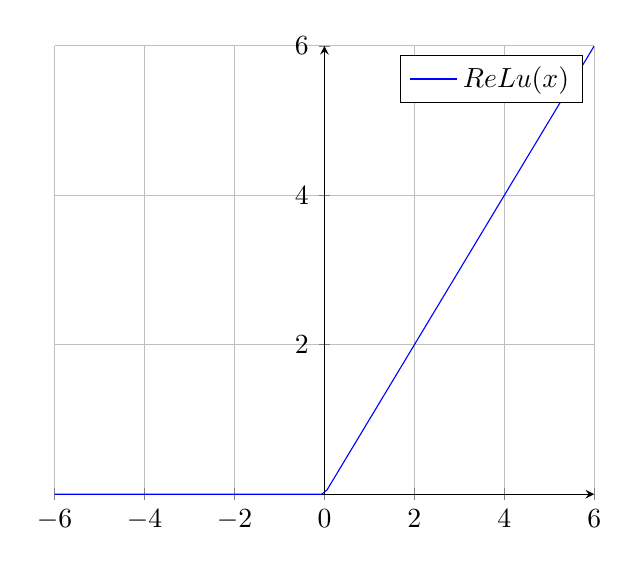
\begin{tikzpicture}[declare function={ReLu(\x)=max(0, x);}]
                        \begin{axis}
                            [
                                grid=major,     
                                axis x line=bottom,
                                ytick={0,2,4,6},
                                axis y line=middle,
                                samples=100,
                                domain=-6:6,
                            ]
                            \addplot[blue,mark=none]   (x,{ReLu(x)});
                            \legend{$ReLu(x)$}
                        \end{axis}
                        \end{tikzpicture}
                    \end{center}
 
                \paragraph{Leaky ReLu} \mbox{} \\
                \begin{center}
                    \[
                        \text{ReLu}(x) =  \begin{cases}
                                            x < 0 & 0.1 \times x \\
                                            x > 0 & x
                                            \end{cases}
                    \]
                    
                    \vspace{0.2cm}
                    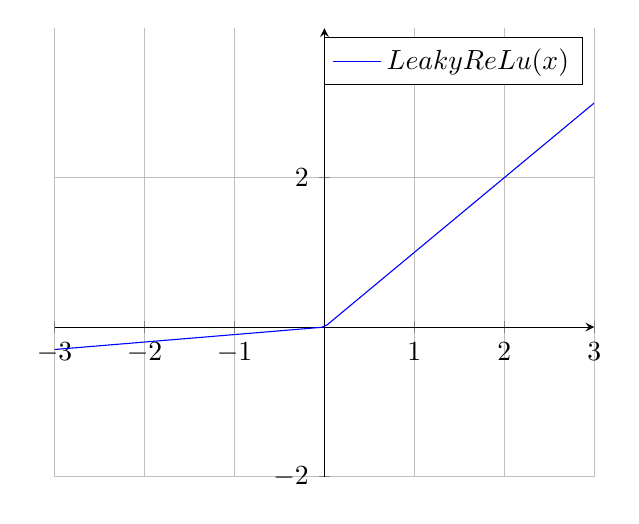
\begin{tikzpicture}[declare function={LeakyReLu(\x)=max(0.1*x, x);}]
                    \begin{axis}
                        [
                            grid=major,     
                            ytick={-2,0,2},
                            axis x line=middle,
                            axis y line=middle,
                            samples=100,
                            domain=-3:3,
                            ymin=-2,
                            ymax=4,
                        ]
                        \addplot[blue,mark=none]   (x,{LeakyReLu(x)});
                        \legend{$LeakyReLu(x)$}
                    \end{axis}
                    \end{tikzpicture}
                \end{center}

                \paragraph{Sigmoid} \mbox{} \\
                    \begin{center}
                        Sigmoid$(x) = $ \mathLarge{\frac{1}{1 + e^{-x}}} \\
                        \vspace{0.2cm}
                        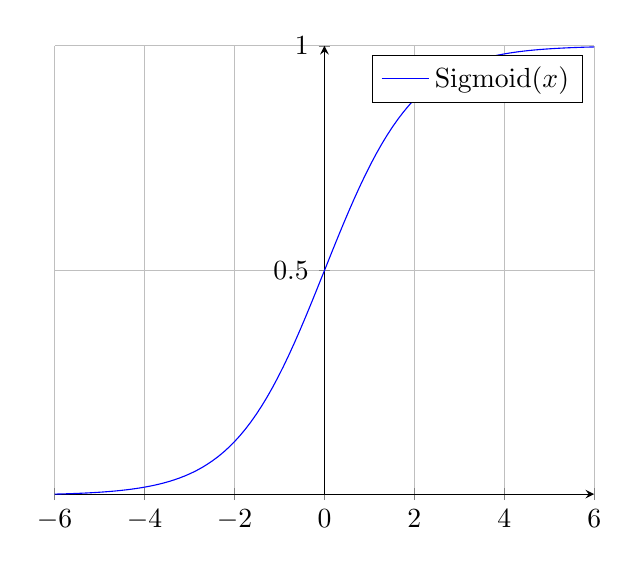
\begin{tikzpicture}[declare function={sigma(\x)=1/(1+exp(-\x));}]
                        \begin{axis}
                            [
                                grid=major,     
                                axis x line=bottom,
                                ytick={-1,-.5,0,.5,1},
                                ymax=1,
                                axis y line=middle,
                                samples=100,
                                domain=-6:6,
                                range=-1:1
                                legend style={at={(1,0.9)}}     
                            ]
                                \addplot[blue,mark=none]   (x,{sigma(x)});
                                \legend{Sigmoid$(x)$}
                        \end{axis}
                        \end{tikzpicture}
                    \end{center}

                \paragraph{TanH} \mbox{} \\
                    \begin{center}
                        TanH$(x) = $ \mathLarge{\frac{\sinh(x)}{\cosh(x)}} $ = $ \mathLarge{\frac{e^{x} - e^{-x}}{e^{x} + e^{-x}}} \\
                        \vspace{0.4cm}
                        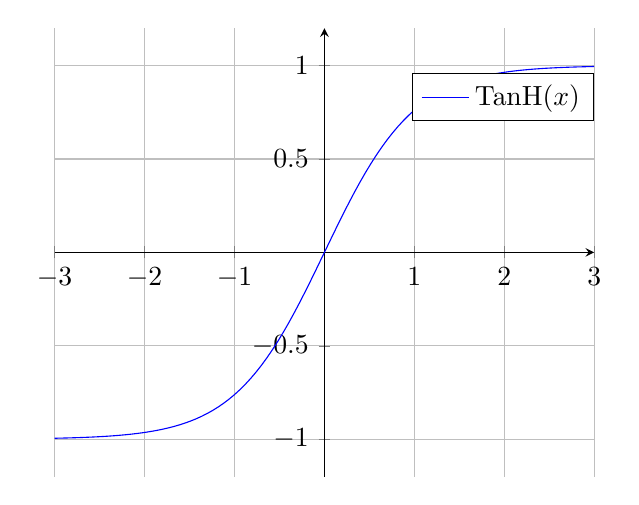
\begin{tikzpicture}[declare function={TanH(\x)=(exp(\x) - exp(-\x))/(exp(\x) + exp(-\x));}]
                        \begin{axis}
                            [
                                grid=major,     
                                axis x line=middle,
                                ytick={-1,-.5,0,.5,1},
                                axis y line=middle,
                                samples=100,
                                domain=-3:3,
                                ymax=1.2,
                                ymin=-1.2,
                                legend style={at={(1,0.9)}}     
                            ]
                                \addplot[blue,mark=none] (x,{TanH(x)});
                                \legend{TanH$(x)$}
                        \end{axis}
                        \end{tikzpicture}
                    \end{center}

                \paragraph{SoftMax} \mbox{} \\
                    SoftMax is an exception to the Activation Functions and is a Generalisation of Sigmoid to Multiple Dimensions. It
                    takes in a Vector \textbf{z} of $K$ Real Numbers, and normalises it into a probability distribution which Sums to 1. \\ 

                    \begin{center}
                        \begin{math}
                            \text{SoftMax}(\textbf{z})_{i} = \mathLarge{\frac{e^{z_{i}}}{\sum_{j=1}^{K} e^{z_{j}}}}
                        \end{math} \\
                        \vspace{0.2cm}
                        For $i = 1, \hdots,K$ And \textbf{z} $ = (z_{1},\hdots,z_{K})$ \\
                    \end{center}
                    
            \subsubsection{Differentiation}
                \paragraph{Differentiation from First Principles}  \mbox{} \\
                    \vspace{0.2cm}
                    Differentiation is the process of finding the Gradient of a Function at a specific point. In the case of a Neural Network,
                    this can be used to measure the sensitivity of the Function Output, in respect to the Input. This derivative is known as said 
                    Functions' Gradient Function. \\
                    \vspace{0.2cm}
                    
                    With a simple straight line graph we can find the gradient as {\Large$\frac{\Delta y}{\Delta x}$, $\Delta$} (Delta) is used to 
                    represent a fininite increment. \\
                    \vspace{0.2cm}

                    When find the Derivative of a more Complex Function we can use Two Points. Point $P : (x, f(x))$ and Point $Q : (x + h, f(x + h))$.
                    The variable $h$ tends towards 0, so Points $Q$ will eventually be ontop of point $P$. This is called Differentiation from First
                    Principles.
                    \vspace{0.4cm}

                    \begin{eqnarray*}
                        \frac{\Delta y}{\Delta x} &=& \lim_{h\to0} \left(\frac{f(x + h) - f(x)}{(x + h) - x}\right) \\
                        &=& \lim_{h\to0} \left(\frac{f(x + h) - f(x)}{h}\right)
                    \end{eqnarray*}
                    \vspace{0.6cm}

                    Derivatives are more commonly represented as $f'(x)$ or $\frac{dy}{dx}$

                    \vspace{0.4cm}
                \paragraph{Standard Differentiation Rules}  \mbox{} \\
                    \vspace{0.2cm}
                    Instead of manually using Smaller and Smaller Values of $h$ manually, there are standard Differentiation Rules. These are as follows: \\
                    \vspace{0.4cm}

                    \begin{eqnarray*}
                        y = x^{k} &\rightarrow& \frac{dy}{dx} = kx^{k-1} \\
                        y = k &\rightarrow& \frac{dy}{dx} = 0 \\
                        y = e^{kx} &\rightarrow& \frac{dy}{dx} = ke^{kx} \\
                        y = f(x)g(x) &\rightarrow& f(x)g'(x) + f'(x)g(x) \\
                        f(x) = \frac{g(x)}{h(x)} &\rightarrow& f'(x) = \frac{g'(x)h(x) - g(x)h'(x)}{h(x)^{2}} \\
                    \end{eqnarray*}
                    \vspace{0.4cm}

                    These rules are applied to each component of the Function to find the Derivative. 

                \paragraph{Chain Rule}  \mbox{} \\
                    \vspace{0.2cm}
                    The Chain Rule is used to compute the derivative of Nested Functions such as $f(x) = g(h(x))$. The derivative of this Function can be expressed as: \\
                    \vspace{0.4cm}

                    \[f'(x) =  g'(h(x))h'(x)\]

                    \vspace{0.4cm}

                    This can be applied to an infinite number of Functions, where $f(x) = g_{1}(g_{2}(\hdots(g_{n}(x))))$. By this rule we can represent the derivative as
                    a Series of Derivatives Multiplied together:

                    \[
                        \frac{df}{dx} = \frac{df}{df_{1}} \frac{df_{1}}{df_{2}} \frac{df_{2}}{df_{3}} \hdots \frac{df_{n}}{df_{x}}
                    \]

                \paragraph{Partial Derivatives}  \mbox{} \\
                    \vspace{0.2cm}
                    Partial Derivatives are used when the Function in question contains Multiple Variables. They utilise the same rules, except the Variables
                    which aren't being derived get treated as constants. The Derivative of $f(x, y)$ with respect to $x$ is expressed as $f_{x}'(x,y)$ or 
                    {\Large $\frac{\partial f}{\partial x}$}. 

            \subsubsection{Back Propagation}
                \paragraph{Overview} \mbox{} \\
                    \vspace{0.2cm}
                    Back Propagation is the algorithm used to adjust Weights and Bias' in a Neural Network. Through using this algorithm you can successfully "train"
                    the Network to recognise certain patterns in data. The Input Data gets propagated through the Network using Forward Propagation, and then the output
                    is passed into the Loss Function.

                \paragraph{The Bellman Equation} \mbox{} \\
                    \vspace{0.2cm}
                    The Bellman Equation is a method of optimisation, and is used for dynamic programming. In the context of Machine Learning we can utilise it
                    to reinforce good behaviour and negate bad behaviour. By writing the relationships between two states in the form of an action, we can optimise this
                    by choosing the best action when given a state. If we let $s_{t}$ be the current state, we can define all the possible actions from that state as
                    $a_{t} \in \Gamma(s_{t})$. Where $\Gamma(s_{t})$ represents all given actions from a state. We can also define the State Transition from $s_{t} \to s_{t+1}$ 
                    as $T(s_{t}, a)$ when action $a$ has been taken. The Reward from this is given as $R(s_{t}, a)$. A Discount Factor $0 < \gamma < 1$ is also defined to assume
                    impatience, compounding the effects of $\gamma$ the further in the future the Reward is. \\
                    \vspace{0.2cm}
                    With these definitions, an infinite-horizon problem is formed: \\

                    \[ V(s_{0}) = \max_{\{a_{t}\}_{t=0}^{\infty}} \sum_{t=0}^{\infty} \gamma^{t} \cdot R(s_{t},a_{t}) \]
                    \vspace{0.2cm}

                    We can form this into another Equation which uses the Principle of Optimality, such that: \\
                    \vspace{0.2cm}

                    \begin{center}
                        \textit{An optimal policy has the property that whatever the initial state and initial decision are, the remaining decisions must constitute an 
                        optimal policy with regard to the state resulting from the first decision.} - Richard E. Bellman
                    \end{center}
                    \vspace{0.2cm}

                    We will consider the first decision seperately to all future reward, and then collect the future decisions within the brackets, which the infinite-horizon problem
                    above is equivalent too.

                    \[ \max_{a_{0}} \left\{ R(s_0, a_0) + \gamma \cdot \left[ \max_{\{a_{t}\}_{t=1}^{\infty}} \sum_{t=1}^{\infty} \gamma^{t-1} \cdot R(s_{t},a_{t})\right] \right\} \]
                    \vspace{0.2cm}

                    This at first glance has only made the problem uglier but infact has made our lives easier. It can be condensed further into a Recursively Defined Function:
                    \vspace{0.2cm}

                    \[ V(s_{0}) = \max_{a_{0}} \{ R(s_{0}, a_{0}) + \gamma \cdot V(x_{1}) \} \] 
                    \centerline{When subjected to: $ x_{1} = T(s_{0}, a_{0})$}
                    \vspace{0.2cm}

                \paragraph{Loss Function} \mbox{} \\
                    \vspace{0.2cm}
                    The Loss Function of a Network represents how well a Neural Network is performing. The aim of the Back Propagation is to minimise this Functions output. When using
                    a standard Neural Network and you're training on a labelled data set, you can be certain about the Expected Output. The standard Loss Function is as follows: \\ 
                    \vspace{0.2cm}
                    
                    \begin{eqnarray*}
                        Loss_{i} &=& \frac{1}{2} \cdot (Expected Output_{i} - Actual Output_{i})^{2} \\
                        &=& \frac{1}{2} \cdot (y_{i} - \hat{y}_{i})^{2}
                    \end{eqnarray*}
                    \vspace{0.2cm}

                    This is whats called the Half Square Difference. This Differentiates nicely which is why it is commonly used. \\
                    \vspace{0.2cm}

                    We use the Bellman Equation to calculate the expected value for the loss function.: \\
                    \vspace{0.2cm}

                    \[Q(s_t, a_t) = R(s_t, a_t) + \gamma \cdot \max_{a_{t+1}} Q(s_{t+1}, a_{t+1})\]
                    \[y = \left( R(s_t, a_t) + \gamma \cdot \max_{a_{t+1}} Q(s_{t+1}, a_{t+1}) - Q(s_t, a_t) \right)^2\]

                \paragraph{Gradient Descent} \mbox{} \\ 
                    \vspace{0.2cm}   
                    To minimise the Loss Function, the Weights and Bias' in the Network need to be algorithmically adjusted to converge towards the expected outputs. You can
                    calculate these adjustments by using Partial Derivatives. You can take the Derivative of every Weight and Bias with respect to the Loss Function. The Derivatives
                    of each weight can vary, such as one weight being 0.5 and the other being 3, the Second Weight affects the Loss Function 10$\times$ as much. This process is
                    known as Gradient Descent. \\

                \paragraph{Differentiating Activation Functions} \mbox{} \\ 
                    \vspace{0.2cm}
                    As part of Back Propgation we need to derive all the Activation Functions we use within our Layer structure. The Derivatives are shown below. \\
                    \vspace{0.2cm}
                    The ReLu Derivative:
                    \vspace{0.2cm}
                    \[
                        \text{ReLu}(x) =  \begin{cases}
                                            0 & x < 0 \\
                                            x & x > 0
                                            \end{cases} 
                    \]
                    \[
                        \text{Relu'}(x) = \begin{cases}
                                            0 & x < 0 \\
                                            1 & x > 0
                                            \end{cases}
                    \]
                    \vspace{0.2cm}
                    \begin{center}
                        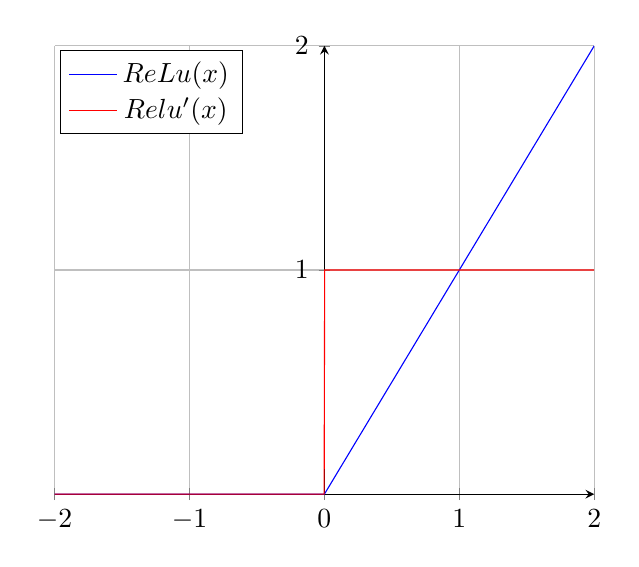
\begin{tikzpicture}[declare function={ReLu(\x)=max(0, x);}]
                        \begin{axis}
                            [
                                grid=major,     
                                axis x line=bottom,
                                ytick={0,1,2,3,4},
                                axis y line=middle,
                                samples=1000,
                                domain=-2:2,
                                legend style={at={(0.01,0.99)},anchor=north west},
                                ymax=2,
                                ymin=0,
                            ]
                            \addplot[blue,mark=none]   (x,{ReLu(x)});
                            \addplot [red,mark=none] {ifthenelse(x>0,1,0)};
                            \legend{$ReLu(x)$, $Relu'(x)$}
                        \end{axis}
                        \end{tikzpicture}
                    \end{center}

                    The Sigmoid Function Derivative:
                    \vspace{0.2cm}
                    \begin{eqnarray*}
                        \text{Sigmoid}(x) &=& \mathLarge{\frac{1}{1 + e^{-x}}} \\
                                            &=& (1 + e^{-x})^{-1} \\
                        \frac{d\sigma(x)}{dx}&=& -1 \cdot (1 + e^{-x})^{-2} \cdot -e^{-x} \\
                                            &=& \mathLarge{\frac{e^{-x}}{(1 + e^{-x})^{2}}} \\
                                            &=& \mathLarge{\frac{e^{-x}}{1 + e^{-x}} \cdot \frac{1}{1 + e^{-x}}} \\
                                            &=& \mathLarge{\frac{e^{-x} + 1 - 1}{1 + e^{-x}} \cdot \frac{1}{1 + e^{-x}}} \\
                                            &=& \left( \mathLarge{\frac{1 + e^{-x}}{1 + e^{-x}} - \frac{1}{1 + e^{-x}}} \right) \cdot \mathLarge{\frac{1}{1 + e^{-x}}} \\
                                            &=& \text{Sigmoid}(x) \cdot (1 - \text{Sigmoid}(x)) \\
                    \end{eqnarray*}
                    
                    \vspace{0.2cm}
                    \begin{center}
                        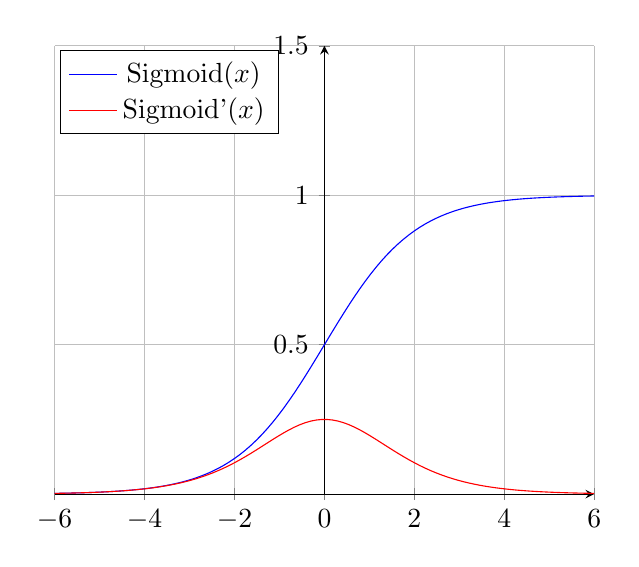
\begin{tikzpicture}[declare function={sigma(\x)=1/(1+exp(-\x));}, declare function={sigmaDer(\x)=sigma(\x)*(1 - sigma(\x));}]
                        \begin{axis}
                            [
                                grid=major,     
                                axis x line=bottom,
                                ytick={-1,-.5,0,.5,1, 1.5},
                                ymax=1.5,
                                ymin=0,
                                axis y line=middle,
                                samples=100,
                                domain=-6:6,
                                legend style={at={(0.01,0.99)},anchor=north west},
                            ]
                                \addplot[blue,mark=none]   (x,{sigma(x)});
                                \addplot[red,mark=none]   (x,{sigmaDer(x)});
                                \legend{Sigmoid$(x)$, Sigmoid'$(x)$}
                        \end{axis}
                        \end{tikzpicture}
                    \end{center}

                    The TanH Derivative:
                    \vspace{0.2cm}
                    \begin{eqnarray*}
                        \text{TanH}(x) &=& \mathLarge{\frac{\sinh(x)}{\cosh(x)}}  \\
                                        &=& \mathLarge{\frac{e^{x} - e^{-x}}{e^{x} + e^{-x}}} \\
                        \text{TanH'}(x)&=& \mathLarge{\frac{(e^{x} + e^{-x})(e^{x} + e^{-x}) - (e^{x} - e^{-x})(e^{x} - e^{-x})}{(e^{x} + e^{-x})^{2}}} \\
                                        &=& \mathLarge{\frac{(e^{x} + e^{-x})^{2}}{(e^{x} + e^{-x})^{2}} - \frac{(e^{x} - e^{-x})^{2}}{(e^{x} + e^{-x})^{2}}} \\
                                        &=& 1 - \text{TanH}^{2}(x) \\
                    \end{eqnarray*}
                    \vspace{0.2cm}

                    \begin{center}
                        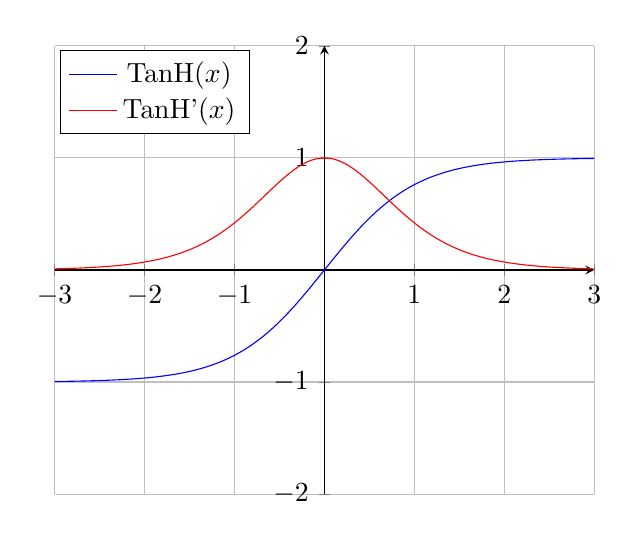
\begin{tikzpicture}[declare function={TanH(\x)=(exp(\x) - exp(-\x))/(exp(\x) + exp(-\x));}, declare function={TanHDer(\x)=1 - TanH(x)^2;}]
                        \begin{axis}
                            [
                                grid=major,     
                                axis x line=middle,
                                ytick={-2,-1,0,1,2},
                                axis y line=middle,
                                samples=100,
                                domain=-3:3,
                                ymax=2,
                                ymin=-2,
                                legend style={at={(0.01,0.99)},anchor=north west}    
                            ]
                                \addplot[blue,mark=none] (x,{TanH(x)});
                                \addplot[red,mark=none] (x,{TanHDer(x)});
                                \legend{TanH$(x)$, TanH'$(x)$}
                        \end{axis}
                        \end{tikzpicture}
                    \end{center}

                \paragraph{Simple Network} \mbox{} \\ 
                    We can apply Back Propagation to this simple Neural Network: \\

                    \centerline{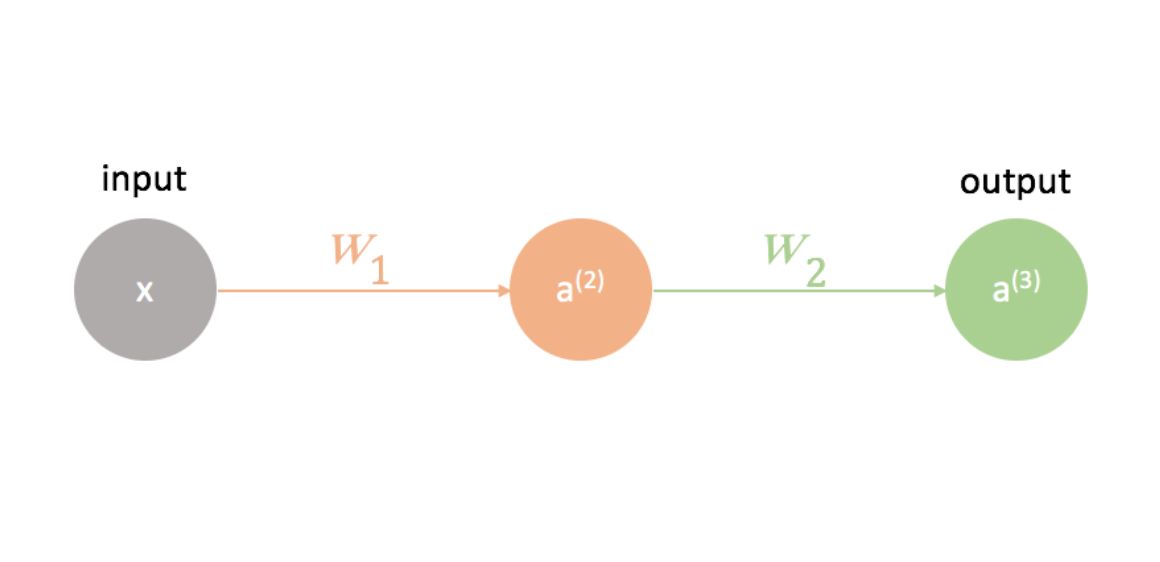
\includegraphics[width=14cm]{Images/ModellingOfProblem/SingleLayerNeuralNetEdited.png}}

                    For this Network we need to calculate the derivative of each weight with respect to the cost function. With
                    the use of the chain rule $w_1$ can be expressed as: \\

                    \[\frac{\partial c}{\partial w_{2}} = \frac{\partial c}{\partial a_3} \frac{\partial a_3}{\partial z_3} \frac{\partial z_3}{\partial w_2}\]

                    This means we need to find each derivative in the chain.
                    \vspace{0.2cm}
                    The first derivative is given as $\mathLarge{\frac{\partial c}{\partial a_3}}$. 
                    \begin{eqnarray*}
                        c &=& \frac{1}{2} \cdot (y - a_3)^2 \\
                        \frac{\partial c}{\partial a_3} &=& y - a_3
                    \end{eqnarray*}
                    Next we find $\mathLarge{\frac{\partial a_3}{\partial z_3}}$, here we will use TanH for our activation function.
                    \begin{eqnarray*}
                        a_3 &=& \frac{e^{z_3} - e^{-z_3}}{e^{z_3} + e^{-z_3}} \\
                            &=& \tanh(z_3) \\
                        \frac{\partial a_3}{\partial z_3} &=& 1 - \tanh^{2}(a_3) \\
                    \end{eqnarray*}
                    Next we find the final derivative $\mathLarge{\frac{\partial z_3}{\partial w_2}}$
                    \begin{eqnarray*}
                        z_3 &=& a_2 \cdot w_2 \\
                        \frac{\partial z_3}{\partial w_2} &=& a_2
                    \end{eqnarray*}
                    We then combine this all together to find $\mathLarge{\frac{\partial c}{\partial w_{2}}}$
                    \begin{eqnarray*}
                        \frac{\partial c}{\partial w_{2}} &=& = (y - a_3) \cdot (1 - \tanh^{2}(a_3)) \cdot a_2
                    \end{eqnarray*}

                    \vspace{0.2cm}

                    When calculating the derivatives of $w_1$ it's slightly more complicated, it requires us to \textit{extend}
                    the chain of derivatives.

                    \[\frac{\partial c}{\partial w_1} = \frac{\partial c}{\partial a_3} \frac{\partial a_3}{\partial z_3} \frac{\partial z_3}{\partial a_2} \frac{\partial a_2}{\partial z_2} \frac{\partial z_2}{\partial w_1}\]

                    It is however similar to our original chain, the only new derivative is $\mathLarge{\frac{\partial z_3}{\partial a_2}}$.
                    Which is simply $w_2$, leaving us with the following derivative:
                    \begin{eqnarray*}
                        \frac{\partial c}{\partial w_{1}} &=& (y - a_3) \cdot (1 - \tanh^{2}(a_3)) \cdot w_2 \cdot a_2 \cdot (1 - \tanh^{2}(a_2)) \cdot a_1
                    \end{eqnarray*}

                    We can generalise this into the form below for layers $1,2, \hdots, n$:
                    \begin{eqnarray*}
                        \frac{\partial c}{\partial w_{l}} &=& a_l \cdot \sigma'(z_{l+1}) \cdot \frac{\partial c}{\partial a_{l+1}} \\
                        \frac{\partial c}{\partial a_{l}} &=&
                        \begin{cases}
                            y - \hat{y} & l = n \\
                            w_l \cdot \sigma'(z_{l+1}) \cdot \frac{\partial c}{\partial a_{l+1}} & Else \\
                        \end{cases} 
                    \end{eqnarray*}

                \paragraph{Complex Network} \mbox{} \\ 
                    For a Complex Network, with multiple Neurons per layer, it is quite similar. An example of this is shown below: \\

                    \centerline{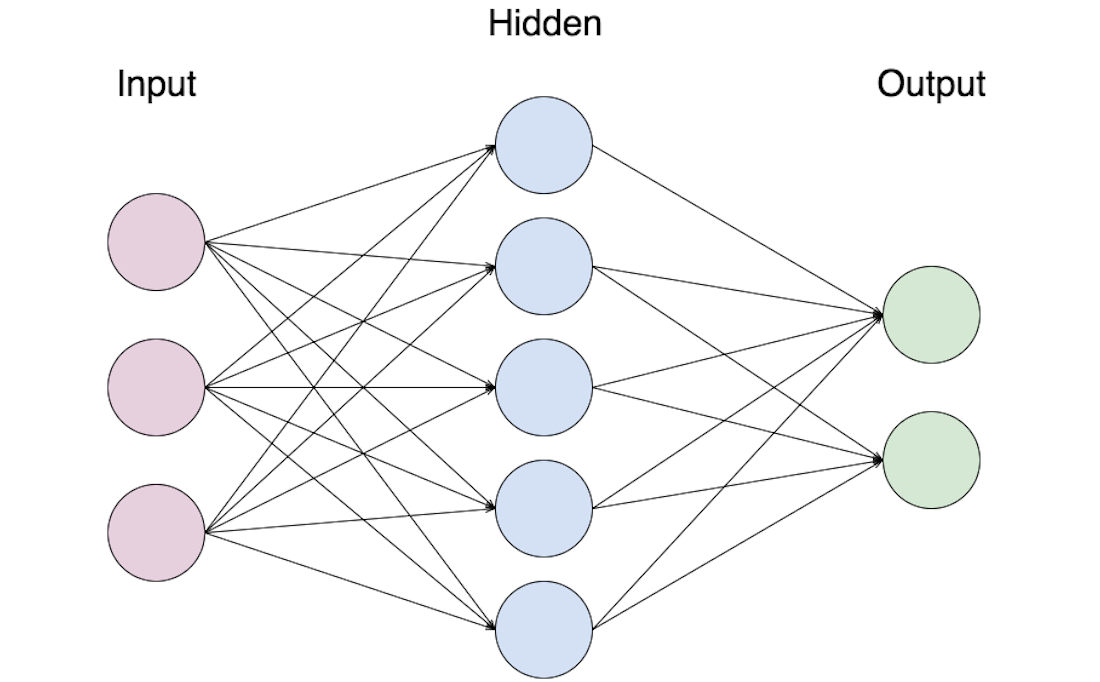
\includegraphics[width=14cm]{Images/InitialResearch/NeuralNetworkExample.png}}

                    When deriving an Activation value we instead need to consider all weight derivatives connected to the next layer. 
                    We can generalise this into the weight update form for layers $1,2, \hdots, n$:
                    \begin{eqnarray*}
                        \Delta w_{i \to j} &=& -\eta\delta_j z_i \\
                        \delta_i &=& 
                        \begin{cases}
                            \sigma'(z_i) \cdot (y_i - \hat{y}_i) & \text{Node $i$ in Final Layer} \\
                            \sigma'(z_i) \sum_{k\in\text{outs}(i)}  \delta_k w_{i \to k} & Else \\
                        \end{cases}
                    \end{eqnarray*}
                    This should be all that is needed to perform Back Propagation.
\end{flushleft}

\begin{flushleft}
    \huge
    \textbf{3. Design}

    \Large
    \begin{enumerate}
        \item {\Large System Flow Charts}
            \large
            \vspace{0.2cm}

        \item {\Large Class Diagrams}
            \large
            \vspace{0.2cm}

        \item {\Large Description of Algorithms}
            \large
            \vspace{0.2cm}
            \begin{enumerate}[label=\arabic*)]
                \item Matrix Addition \\
                This algorithm is a Mathematical Operation to add 2 Matrices together. To Add together 2 Matrices their Orders
                must be the same. To perform the Operation you must Sum each element in Matrix A with the corresponding element 
                in Matrix B, placing the result of each Sum in the resultant Matrix.

                \vspace{0.5cm}
                \item Matrix Subtraction \\
                This algorithm is a Mathematical Operation to subtract 2 Matrices. To Subtract 2 Matrices their Orders
                must be the same. To perform the Operation you must Sum each element in Matrix A with the negative of the 
                corresponding element in Matrix B, placing the result of each Sum in the resultant Matrix.

                \vspace{0.5cm}
                \item Matrix Multiplication \\
                This algorithm is a Mathematical Operation to find the product of 2 Matrices. To Multiply 2 Matrices
                the number of Columns in the Matrix A must be equal to the number of Rows in Matrix B. Where Matrix A has
                dimensions of $m$ x $n$ and Matrix B has dimensions of $j$ x $k$, the resultant Matrix will have dimensions of 
                $n$ x $j$. To Multiply two Matrices, the algorithm performs the Dot Product between the Row in Matrix A and the 
                corresponding Column in Matrix B. The Dot Product is the Sum of the Products of corresponding elements.

                \vspace{0.5cm}
                \item Matrix Scalar Multiplication \\
                This algorithm is a Mathematical Operation to find the product between a Matrix and a Scalar.
                The result can be found by Multiplying each element of the Matrix by the Scalar Value to form the Resultant 
                Matrix.
                
                \vspace{0.5cm}
                \item Matrix Hadamard Product \\
                This algorithm is a Mathematical Operation to another way to find the product between 2 Matrices. Instead of
                applying the Dot Product between Rows and Columns, you find the product between each element in Matrix A
                with the corresponding element in Matrix B, placing the result in the resultant Matrix. This is very epic gamer

                \vspace{0.5cm}
                \item Matrix Power \\
                This algorithm is a Mathematical Operation to find the power of a Matrix. The given Matrix needs to have square dimensions.
                The result can be found by multiplying the given Matrix by itself $n$ ammount of times where $n$ is the given power.
                
                \vspace{0.5cm}
                \item Matrix Transpose \\
                This algorithm is a Mathematical Operation used to Flip a Matrix across its Diagonal. The Transpose of any Matrix
                can be found by converting each Row of the Matrix into a Column. An $m$ x $n$ Matrix will turn into an $n$ x $m$ Matrix.
                
                \vspace{0.5cm}
                \item Activation Function Sigmoid \\
                This algorithm is a Mathematical Formulae which squishes any value to between 0 and 1. It uses Eulers Number $e$.

                \vspace{0.2cm}
                {\Large\centerline{$S(x) = \frac{1}{1 + e^{-x}}$}}
                \vspace{0.2cm}
                
                \vspace{0.5cm}
                \item Activation Function TanH \\
                This algorithm is a Hyperbolic Function which squishes any value to between -1 and 1. It is a Ratio between the two Hyperbolic 
                functions SinH and CosH.

                \vspace{0.2cm}
                {\Large\centerline{$TanH(x) = \frac{SinH(x)}{CosH(x)} = \frac{e^x - e^{-x}}{e^x + e^{-x}}$}}
                \vspace{0.2cm}

                \vspace{0.5cm}
                \item Activation Function Relu \\
                This algorithm is a simple function which removes any negative values from its input, returning 0 instead.
                
                \vspace{0.5cm}
                \item Activation Function SoftMax \\
                This algorithm is a logistic function that creates a probability distribution from a set of points. This probability 
                distribution sums to 1. It applies the standard Exponential Function to each element, then normalises this value by dividing
                by the sum of all these Exponentials.

                \vspace{0.5cm}
                \item Neural Network Forward Propagation \\
                This algorithm is used to obtain the outputs of a Neural Network. It uses Matrix Multiplication to propagate the inputs
                of the network from Layer to Layer, eventually reaching the Output Layer. My Multiplying the Weight Matrix and the outputs
                of the previous Layer, and then adding the Bias. We can obtain the output of the layer.
                
                \vspace{0.5cm}
                \item Neural Network Loss Function \\
                
                
                \vspace{0.5cm}
                \item Neural Network Backwards Propagation \\
                This algorithm is used within a Neural Network to adjust its Weights and Biases, allowing it to more accurately predict the
                best outcome. In Reinforcement Learning, the Network is trained using an estimate for what is the best action given a situation.
                Using this estimate, we can train the Network to predict this outcome by converging the series of Weights and Biases towards a
                local minimum. This is done by calculating partial derivates for every weight and bias value with respect to the cost function.
                This derivative is then subtracted from the existing weight or bias, eventually converging on the best possible value.

                \vspace{0.5cm}
                \item Agent Get Tile Vector \\
                This algorithm takes the current world data of the simulation, and produces a Vector of Tile Data surrounding the Agent. 
                
                \vspace{0.5cm}
                \item Agent Post Process Tile Vector \\
                This algorithm will convert the Tile Vector into a Vector of Grayscale values, which can be used as the input for the Neural
                Network.
                
                \vspace{0.5cm}
                \item Agent Convert to Grayscale \\
                This algorithm converts a given RGB Colour Value to the corresponding Gray Scale Value.

                \vspace{0.5cm}
                \item Agent Spawn Position \\
                This algorithm will create a list of spawnable tiles for which the Agent could spawn on, and then randomnly select a specific
                tile as its spawn position.
                
                \vspace{0.5cm}
                \item Enemy Spawn Position \\
                This algorithm will create a list of spawnable tiles for which Enemies can spawn on, then select tiles randomnly, if they dont
                already contain an enemy or the agent it will create an Enemy Object with that position. It will do this $n$ ammount of times where $n$ is
                the limit to how many enemies can spawn.
                
                \vspace{0.5cm}
                \item Enemy Move \\
                The algorithm I have designed for the Enemy Pathfinding is rather simple, and wont take up much runtime in my solution.
                First it calculates the distance between itself and the Agent in both Axis. The Enemy will then converge upon the Agents
                position by moving in the direction with the greatest distance, effectively finding the nearest diagonal and following it.
                The flow diagram for this Simple Algorithm is shown above under System Flow Charts.
                
                \vspace{0.5cm}
                \item Poisson Disc Sampling \\
                Poisson Disc Sampling is used to sample a set of points in N Dimensional Space. It takes two parameters, $r$ and $k$, where
                $r$ is the minimum distance a specified point must be from every other point, and $k$ is the limit of samples to choose
                before rejection. It starts by creating an N Dimensional Grid which accelerates spacial searches. An initial sample is then
                chosen and inserted into the grid. It then chooses a random point, and determines if it is greater than $r$ range from every 
                other point in the grid. This can easily be acomplished using the previously defined Grid. If after $k$ attempts, no point is
                found then the search is concluded.
                
                \vspace{0.5cm}
                \item Perlin Noise \\
                Perlin Noise is a method of generating a procedural texture depending upon input parameters. It defines an n-dimensional
                grid of Vectors, each grid intersection contains a fixed, random unit vector. To sample Perlin Noise, the grid cell which
                the point lies in must be found. The Vectors between the sampled point, and the corners of the cell. We then take the Dot
                Product between these new Vectors, and the Vectors applied to the intersections. In 2d Space this leaves us with 4 Values.
                We then use an Interpolation function to Interpolate between the 4 Values. 
                
                \vspace{0.5cm}
                \item Octave Perlin Noise \\
                Octave Perlin Noise takes the existing Perlin Noise algorithm, but adds rescaled clones of itself into itself, to create
                what is known as Fractal Noise. Creating this Fractal Noise is common practice because it reduces the sharp edges encountered
                with just the regular Perlin Noise Algorithm.

                \vspace{0.5cm}
            \end{enumerate}

        \item {\Large Description of Data Structures} \\
            \large
            \vspace{0.2cm}
            \begin{enumerate}
                \item {\large Matrices} \\
                As part of developing a Neural Network, I will extensively use Matrices, as they are an integral part of the algorithms
                used for Machine Learning. After creating a prototype Matrix class as part of my prototype, I will represent it in the
                same format. In my prototype I created a Class, and then represented the values of the Matrix with a 2d List (List of Lists).
                As part of my Matrix Class I will have multiple constructors, to help avoid repeating code.
            \end{enumerate}
            

    \end{enumerate}
    \vspace{0.1cm}
\end{flushleft}

\section{Testing}

\subsection{Testing Table}
\subsubsection{Targetted Testing Areas}

\large
As part of testing my NEA, I identified the key areas of my project which needed testing.
My testing targets these areas from different angles to ensure they work correctly. 
These areas are:
\begin{enumerate}
    \item User Input and Program Output
        \begin{enumerate}
            \item Parameter Loading
            \item Neural Network Loading
            \item Graphical Output
            \item Console Output
        \end{enumerate}
    \item Matrix Implementation
        \begin{enumerate}
            \item Constructor Cases
            \item Matrix Operations
            \item Thrown Exceptions
        \end{enumerate}
    \item Deep Q Learning Algorithm
        \begin{enumerate}
            \item Forward Propagation
            \item Loss Function
            \item Back Propagation
            \item Double Ended Queue Data Type
        \end{enumerate}
    \item Data Logger
        \begin{enumerate}
            \item Data Structure Matching
            \item Heap Data Structure
            \item Heap Sort Implementation
        \end{enumerate}
    \item Simulation
        \begin{enumerate}
            \item Generation of 2d Terrain
            \item Continuity of Generation
            \item ML Agent
            \item Reward Methods
        \end{enumerate}
\end{enumerate}

\pagebreak

\begin{center}
    \large
    \textbf{Below is included an NEA Testing video used for some parts of Testing Evidence}
    
    \vspace{0.2cm}
    
    \Large
    \textit{https://thisisalink.com/youtotallybelieveme/}
\end{center}

\vspace{1cm}
\subsubsection{User Input and Program Output Tests}
\vspace{0.5cm}

\normalsize
\begin{longtable}{| C{0.6cm} | C{3cm} | C{4cm} | C{5cm} | L{1cm} | L{1.4cm} |}
    \hline
    {\footnotesize Test No.} & Test Name & Input Data / Description & Expected Output & Pass / Fail & Testing Evidence \\
    \hline\hline
    \rn & Loading Parameters File & Input "Default.json" file which contains the loadable values & Loads parameters into the 
    Parameters Dictionary variable & Pass & 1.1 \\ 
    \hline
    \rn & Parameters within range & Input Loaded Parameters Dictionary & Prints to console "Parameters within Specified Ranges" & Pass & 1.2 \\
    \hline
    \rn & Below Range Parameter & Input "Default.json" file with a below range parameters & Raises an exception detailing the Parameter, 
    Value of Parameters, and the given Range Required & Pass & 1.3 \\
    \hline
    \rn & Above Range Parameter & Input "Default.json" file with an above range parameters & Raises an exception detailing the Parameter, 
    Value of Parameters, and the given Range Required  & Pass & 1.4 \\
    \hline
    \rn & Network Saved Data Loading & When Prompted to load network data type "Y", and type the file name of network data to load & Network 
    Data is loaded successfully, training position stored & Pass & 1.5 \\
    \hline
    \rn & Window Opening & Run Program, enter setup info as normal & Window opens and is of the correct size/resolution & Pass & 1.6 \\
    \hline
    \rn & Window Displays correct debug information & Run Program, enter setup info as normal, with "Debug" = 1 in parameters file & Debug 
    Layer output info displayed on Right side of Window & Pass & 1.7 \\
    \hline
    \rn & Agent is displayed & Run Program, enter setup info as normal & Orange square displayed on screen & Pass & 1.8 \\
    \hline
    \rn & Enemies are displayed & Run Program, enter setup info as normal, with "StartEnemyCount" $\greatereq$ 1  & Red Square/s are displayed 
    on Screen & Pass & 1.9 \\
    \hline
    \rn & Console Messages Output & Run Program, enter setup info as normal & Console Messages Outputted per 100 Steps & Pass & 1.10 \\
    \hline
\end{longtable}

\vspace{1cm}
\setcounter{magicrownumbers}{0}
\subsubsection{Matrix Implementation Tests}
\vspace{0.5cm}

\normalsize
\begin{longtable}{| C{0.6cm} | C{3cm} | C{4cm} | C{5cm} | L{1cm} | L{1.4cm} |}
    \hline
    {\footnotesize Test No.} & Test Name & Input Data / Description & Expected Output & Pass / Fail & Testing Evidence \\
    \hline\hline
    \rn & Create Matrix with Tuple & A Tuple for the order of the Matrix & Matrix is created with an order the same as the Tuple & Pass & 2.1 \\
    \hline
    \rn & Create Matrix with 2d List & A 2d List, where the parent list holds a list for every row, each "row list" is of the same length & Matrix is created with the same values as the 2d List & Pass & 2.2 \\
    \hline
    \rn & Create Vector with List & A 1d List of any Values  & Vector is created with the same values as the List & Pass & 2.3 \\
    \hline
    \rn & Print Matrix to Console & A valid Matrix of any size & Matrix Prints to the console with the correct formatting & Pass & 2.4 \\
    \hline
    \rn & Create Randomised Matrix & A Tuple for the order of the Matrix, and the the keyargument random=True & Matrix is created with randomised values between -0.5 and 0.5 & Pass & 2.5 \\
    \hline
    \rn & Create Identity Matrix & A Tuple for the order of the Matrix, and the the keyargument identity=True & Matrix is created with all 0's and 1's down the diagonal & Pass & 2.6 \\
    \hline
    \rn & Matrix Addition Calculation & Two Matrices of the same order & Matrix Addition is performed to create a new Matrix with the added values & Pass & 2.7 \\
    \hline
    \rn & Matrix Subtraction Calculation & Two Matrices of the same order & Matrix Subtraction is performed to create a new Matrix with the subtracted values & Pass & 2.8 \\
    \hline
    \rn & Matrix Multiplication Calculation & Two Matrices where Width of $M1$ is equal to the height of $M2$ & Matrix Multiplication is performed to create a new Matrix with the multiplied values & Pass & 2.9 \\
    \hline
    \rn & Matrix Scalar Multiplication Calculation & A $float/int$ as the scalar and any size Matrix & Matrix Scalar Multiplication is performed to create a new Matrix with the multiplied values & Pass & 2.10 \\
    \hline
    \rn & Vector Hadamard Product Calculation & Two Vectors with the same Order & Vector Hadamard Product is performed to create a new Vector with the multiplied values & Pass & 2.11 \\
    \hline
    \rn & Matrix Power Calulation & A Square Matrix with values stored in it & Matrix to the Power of is performed to create a new Matrix with the correct values & Pass & 2.12 \\
    \hline
    \rn & Matrix Transpose Calculation & A Matrix with values stored in it & New Matrix is created with values flipped across the diagonal & Pass & 2.13 \\
    \hline
    \rn & Matrix Select Column & A Matrix with values stored in it & Selects the indexed Column from the Matrix, returning as a list & Pass & 2.14 \\
    \hline
    \rn & Matrix Select Row & A Matrix with values stored in it & Selects the indexed Row from the Matrix, returning as a list & Pass & 2.15 \\
    \hline
    \rn & Vector Max in Vector & A Vector & Returns Largest value in Vector & Pass & 2.16 \\
    \hline
    \rn & Matrix Clear & A Matrix with values stored in it & Clears Matrix of any values & Pass & 2.17 \\
    \hline
    \rn & Combine Vectors & List of Vectors of the same Order & Combines the list of Vectors into a Matrix & Pass & 2.18 \\
    \hline
    \rn & Matrix Sum & - & Sums all values in the Matrix returning a $float/int$ & Pass & 2.19 \\
    \hline
    \rn & Randomised Matrix Constructor Tests & Generator Constructor Parameters randomnly for 10000 Tests & All Tests Should produce a valid Matrix & Pass & 2.16 \\
    \hline
    \rn & Randomised Constructor Exception Tests & Generate Random Data to cause Exceptions within the Constructor for 10000 Tests & All Tests should 
    trigger the Targetted Exception for that test & Pass & 2.17 \\
    \hline
    \rn & Randomised Operator Tests & Generator Random Data to test the Operator Methods for 10000 Tests & All Tests should produce the correct result & Pass & 2.18 \\
    \hline
    \rn & Randomised Operator Exception Tests & Generate Random Data to cause Exceptions within the Operators for 10000 Tests & All Tests should 
    trigger the Targetted Exception for that test & Pass & 2.19 \\
    \hline
\end{longtable}

\vspace{1cm}
\setcounter{magicrownumbers}{0}
\subsubsection{Deep Reinforcement Learning Algorithm Tests}
\vspace{0.5cm}

\small
\begin{longtable}{| C{0.6cm} | C{3cm} | C{4cm} | C{5cm} | L{1cm} | L{1.4cm} |}
\hline
{\footnotesize Test No.} & Test Name & Input Data / Description & Expected Output & Pass / Fail & Testing Evidence \\
    \hline\hline
    \rn & Networks are Created & Run Program, enter setup info, denying the loading of weights & A Dual Neural Network is created after Program Start & Pass & 3.1 \\
    \hline
    \rn & Networks conforms to Parameters & Run Program, enter setup info, denying the loading of weights & The created Dual Neural Network conforms to the specified structure 
    in the parameter "DeepQLearningLayers" & Pass & 3.2 \\
    \hline
    \rn & Forward Propagation Test & Run program as normal & Actions are predicted by the Network & Pass & 3.3 \\
    \hline
    \rn & Loss Function & Run program as normal & Loss is calculated & Pass & 3.4 \\
    \hline
    \rn & Back Propagation Test & Run program as normal & Calculated Loss is Back Propagated through the Network & Pass & 3.5 \\
    \hline
    \rn & Deque Push Front & A value to push to the Deque & Item is pushed to front of Deque & Pass & 3.6 \\
    \hline
    \rn & Deque First/Last & Call the .First() or .Last() Method for a Deque Object & Returns item at Front/Last index of Deque & Pass & 3.7 \\
    \hline
    \rn & Deque Sample N Ammount of Items & Call the .Sample(int N) Method, with a parameter of N items, for a Deque Object & Returns N number of random 
    samples from Deque & Pass & 3.8 \\
    \hline
    \rn & Experience Replay Sampling & Run program as normal & Back Propagation is performed on the sampled Deque Items & Pass & 3.9 \\
    \hline
    \rn & Activation Outputs Unit Test & Input Value Vector to the Activation Function & Returns a Vector of values, where the Activation has been 
    applied to them & Pass & 3.10 \\
    \hline
    \rn & Activation Derivatives Output Unit Test & Input Value Vector to the Activation Derivative Function & Returns a Vector of values, where the 
    Activation Deivative has been applied to them & Pass & 3.11 \\
    \hline
\end{longtable}

\vspace{1cm}
\setcounter{magicrownumbers}{0}
\subsubsection{Data Logger Tests}
\vspace{0.5cm}

\normalsize
\begin{longtable}{| C{0.6cm} | C{3cm} | C{4cm} | C{5cm} | L{1cm} | L{1.4cm} |}
\hline
{\footnotesize Test No.} & Test Name & Input Data / Description & Expected Output & Pass / Fail & Testing Evidence \\
    \hline\hline
    \rn & Heap Sort Decending & A randomnly generated input list & Sorts the list of items into Descending order & Pass & 4.1 \\
    \hline
    \rn & Add Point & A Data Point matching the data structure of the DataCollector & Point is added to Data Points list & Pass & 4.2 \\
    \hline
    \rn & Match Data Struture with Single & Data Structure contrains an index with a Single-Typed 
    definition & No error thrown & Pass & 4.3 \\
    \hline
    \rn & Match Data Struture with Multi-Typed & Data Structure contrains an index with a Multi-Typed
    definition & No error thrown & Pass & 4.4 \\
    \hline
    \rn & Match Data Struture with List-Typed & Data Structure contrains an index with a List-Typed 
    definition & No error thrown & Pass & 4.5 \\
    \hline
    \rn & Match Data Structure Error & Try match point with structure which does not match & Error is thrown with correct info & Pass & 4.6 \\
    \hline
    \rn & Select Query & Select from DataLogger with an Index and Search Contents & Returns a list of the selected column where the Search Contents Matches & Pass & 4.7 \\
    \hline
    \rn & Save Data Points & Invoke Save method on DataLogger Object & Saves Data Points to specified File & Pass & 4.8 \\
    \hline
    \rn & Load Data Points & Invoke Load method on DataLogger Object & Loads Data Points from specified File & Pass & 4.9 \\
    \hline
\end{longtable}

\vspace{1cm}
\setcounter{magicrownumbers}{0}
\subsubsection{Simulation Tests}
\vspace{0.5cm}

\normalsize
\begin{longtable}{| C{0.6cm} | C{3cm} | C{4cm} | C{5cm} | L{1cm} | L{1.4cm} |}
\hline
{\footnotesize Test No.} & Test Name & Input Data / Description & Expected Output & Pass / Fail & Testing Evidence \\
    \hline\hline
    \rn & Creation of Agent & Run progam as normal & Agent is created as an instance of the Agent Class & Pass & 5.1 \\
    \hline
    \rn & Creation of Enemies & Run program as normal with the "StartEnemyCount" Parameter $\greatereq 1$ & Up to the ammount of specified Enemies are created & Pass & 5.2 \\
    \hline
    \rn & Enemies Pathfind towards Agent & Run program as normal with "StartEnemyCount" Parameter $\greatereq 1$ & The spawned enemies pathfind towards the agent 
    using the defined pathfinding algorithm & - & - \\
    \hline
    \rn & Getting Tile Data & Call .GetTileVector(worldMap, enemyList[]) with arguments for worldMap and the list of current Enemies & Returns a Vector of the 
    surrounding tile objects & Pass & 5.4 \\
    \hline
    \rn & Convert Tile Data & Call .TileVectorPostProcess(tileVec) with argument of the result from the Test Above & Converts Tile Data into two vectors, Grayscale 
    Colour and Tile Type & Pass & 5.5 \\
    \hline
    \rn & Reward System Test & Program running as normal & Expected reward is given to agent & Pass & 5.6 \\
    \hline
    \rn & World Generates to an Acceptable Standard & Run program as normal & Generates 2d Terrain which roughly looks realistic & Pass & 5.7 \\
    \hline
    \rn & World Generation Conforms to Parameters & Utilise inputted parameters to identify the effect they have on the world Generation & Terrain changes depending on inputting Parameters & Pass & 5.8 \\
    \hline
    \rn & Perlin Noise retains Continuity & Generate two worlds with the same seed & Perlin Noise returns same value when using the same seed twice & Pass & 5.9 \\
    \hline
\end{longtable}

\pagebreak
\vspace{1cm}
\subsection{Testing Evidence}
\vspace{0.5cm}

\subsubsection{User Input and Program Output Evidence}

\setcounter{magicrownumbers}{0}
\normalsize
\begin{center}
    {\large Evidence 1.\rn }\\ 
    \vspace{0.3cm}
    The .json file which is being loaded \\
    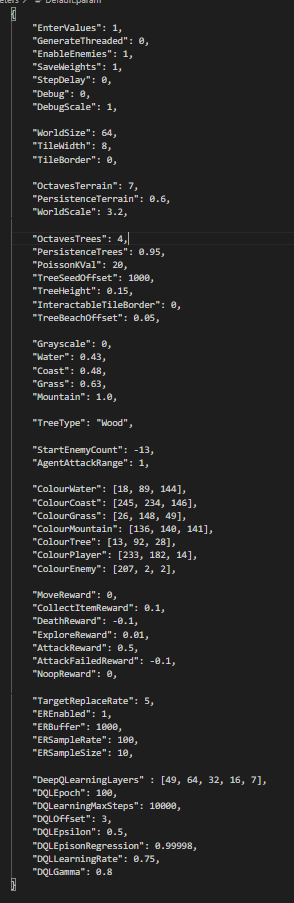
\includegraphics[width=6cm]{Images/Testing/T1.1.1.PNG} \\
    Printing the loaded Json File to console to Console to check the values match\\
    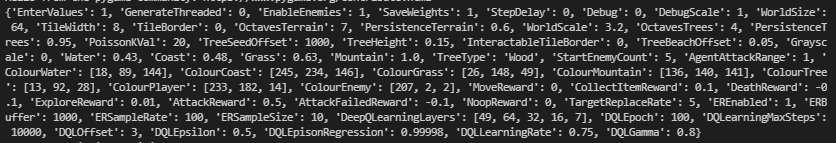
\includegraphics[width=16cm]{Images/Testing/T1.1.2.PNG} \\
    \vspace{1cm}

    {\large Evidence 1.\rn } \\ 
    \vspace{0.3cm}
    Console Output when parameters are within specified ranges \\
    
\includegraphics[width=6cm]{Images/Testing/T1.2.1.PNG} \\
    A Screenshot of the .json file where the Ranges are defined \\
    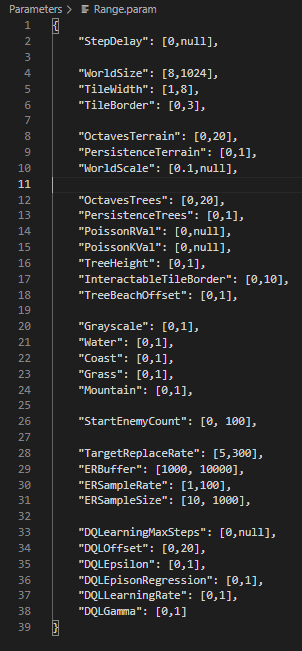
\includegraphics[width=6cm]{Images/Testing/T1.2.2.PNG}
    \vspace{1cm}

    {\large Evidence 1.\rn } \\ 
    \vspace{0.3cm}
    The given out of range parameter - subceeding \\
    
\includegraphics[width=6cm]{Images/Testing/T1.3.1.PNG} \\
    The specified range it should be within \\
    
\includegraphics[width=6cm]{Images/Testing/T1.3.2.PNG} \\
    The Exception thrown when the program is run \\
    
\includegraphics[width=12cm]{Images/Testing/T1.3.3.PNG} \\
    \vspace{1cm}

    {\large Evidence 1.\rn }\\ 
    \vspace{0.3cm}
    The given out of range parameter - exceeding \\
    
\includegraphics[width=6cm]{Images/Testing/T1.4.1.PNG} \\
    The specified range it should be within \\
    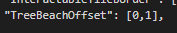
\includegraphics[width=6cm]{Images/Testing/T1.4.2.PNG} \\
    The Exception thrown when the program is run \\
    
\includegraphics[width=12cm]{Images/Testing/T1.4.3.PNG} \\
    \vspace{1cm}

    {\large Evidence 1.\rn }\\ 
    \vspace{0.3cm}
    The Console prompt if the user wants to load Network Weights \\
    
\includegraphics[width=6cm]{Images/Testing/T1.5.1.PNG} \\
    The file the program is loading \\
    
\includegraphics[width=4cm]{Images/Testing/T1.5.2.PNG} \\
    The testing step resumes at 400, underlined in Red \\
    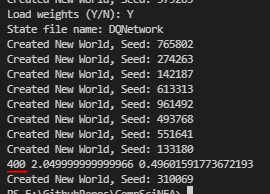
\includegraphics[width=6cm]{Images/Testing/T1.5.3.PNG}
    \vspace{1cm}

    {\large Evidence 1.\rn } \\ 
    \vspace{0.3cm}
    The width/height of the window\\
    
\includegraphics[width=4cm]{Images/Testing/T1.6.1.PNG} \\
    The opened window, it is 64 wide and 64 tall \\
    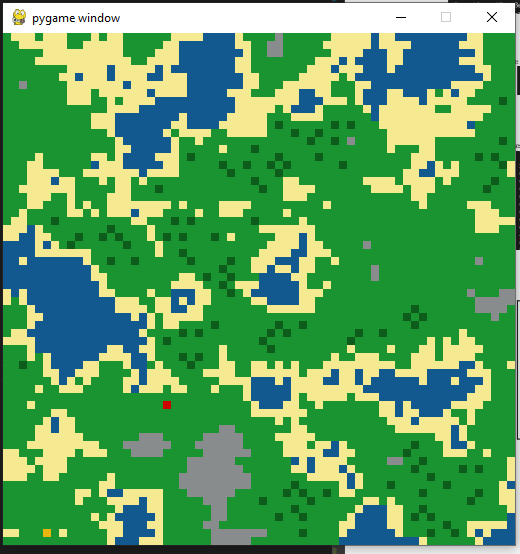
\includegraphics[width=8cm]{Images/Testing/T1.6.2.PNG}
    \vspace{1cm}

    {\large Evidence 1.\rn } \\ 
    \vspace{0.3cm}
    Debug being set to 1 in the parameters file \\
    
\includegraphics[width=4cm]{Images/Testing/T1.7.1.PNG} \\
    The displayed debug information to the right of the Window \\
    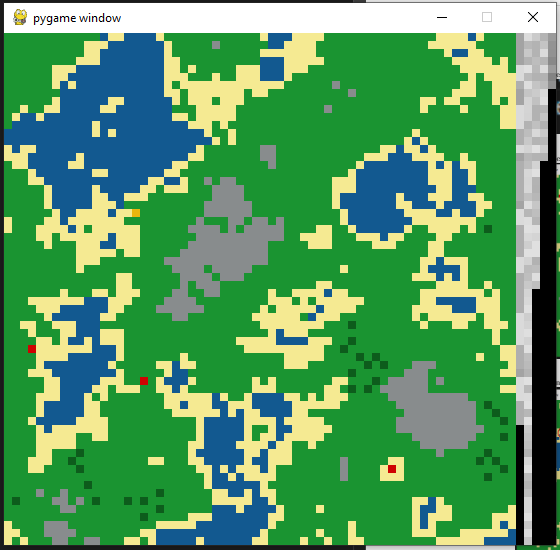
\includegraphics[width=8cm]{Images/Testing/T1.7.2.PNG} \\
    \vspace{1cm}

    {\large Evidence 1.\rn } \\ 
    \vspace{0.3cm}
    The opened window, with the agent circled \\
    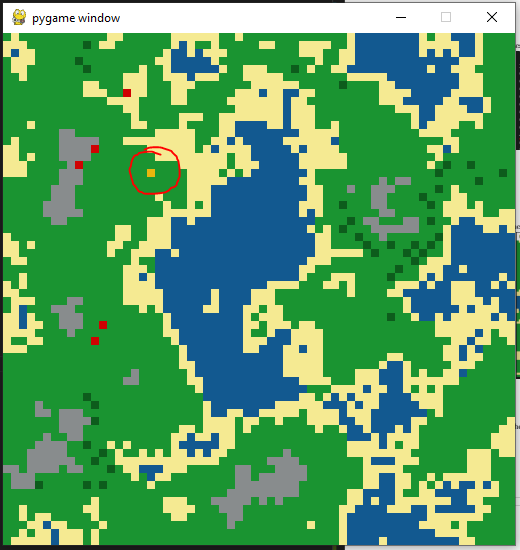
\includegraphics[width=8cm]{Images/Testing/T1.8.1.PNG} \\
    \vspace{1cm}

    {\large Evidence 1.\rn } \\ 
    \vspace{0.3cm}
    The opened window, with the enemies circled \\
    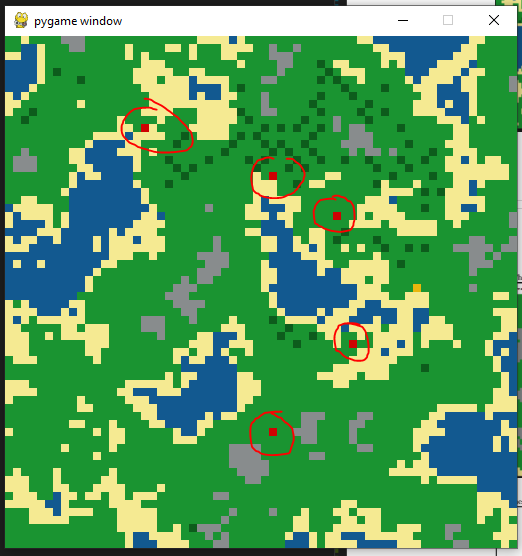
\includegraphics[width=8cm]{Images/Testing/T1.9.1.PNG} \\
    \vspace{1cm}

    {\large Evidence 1.\rn } \\ 
    \vspace{0.3cm}
    The correctly displayed console outputs \\
    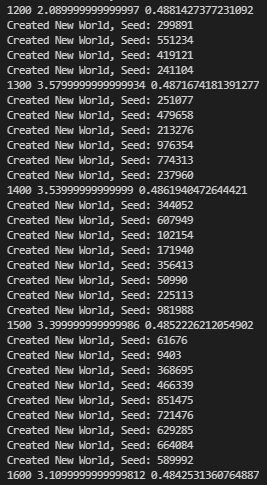
\includegraphics[width=8cm]{Images/Testing/T1.10.1.PNG} \\
\end{center}

\subsubsection{Matrix Implementation Tests}

\setcounter{magicrownumbers}{0}
\begin{center}
    {\large Evidence 2.\rn } \\ 
    \vspace{0.3cm}
    Creating a Matrix with a Tuple \\
    \begin{pythoncode}
matrix = Matrix((3, 4))
print(matrix)
    \end{pythoncode}
    The output of the above code: \\
    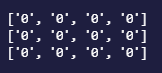
\includegraphics[width=3cm]{Images/Testing/T2.1.1.PNG} \\
    \vspace{1cm}

    {\large Evidence 2.\rn } \\ 
    \vspace{0.3cm}
    Creating a Matrix with a 2d List \\
    \begin{pythoncode}
values = [[3, 4],
        [1, 2]]
matrix = Matrix(values)
print(matrix)
    \end{pythoncode}
    The output of the above code: \\
    
\includegraphics[width=3cm]{Images/Testing/T2.2.1.PNG} \\
    \vspace{1cm}

    {\large Evidence 2.\rn } \\ 
    \vspace{0.3cm}
    Creating a Matrix with a 1d List \\
    \begin{pythoncode}
values = [1, 2, 3, 4]
matrix = Matrix(values)
print(matrix)
    \end{pythoncode}
    The output of the above code: \\
    
\includegraphics[width=1.5cm]{Images/Testing/T2.3.1.PNG} \\
    \vspace{1cm}

    {\large Evidence 2.\rn } \\ 
    \vspace{0.3cm}
    Printing a Matrix to the console \\
    \begin{pythoncode}
values = [[4, 3],
        [2, 1]]
matrix = Matrix(values)
print(matrix)
    \end{pythoncode}
    The output of the above code: \\
    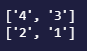
\includegraphics[width=3cm]{Images/Testing/T2.4.1.PNG} \\
    \vspace{1cm}

    {\large Evidence 2.\rn } \\ 
    \vspace{0.3cm}
    Creating a Randomised Matrix \\
    \begin{pythoncode}
matrix = Matrix((2, 2), random=True)
print(matrix)
    \end{pythoncode}
    The output of the above code: \\
    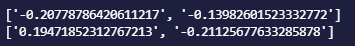
\includegraphics[width=8cm]{Images/Testing/T2.5.1.PNG} \\
    \vspace{1cm}

    {\large Evidence 2.\rn } \\ 
    \vspace{0.3cm}
    Creating an Identity Matrix \\
    \begin{pythoncode}
matrix = Matrix((3, 3), identity=True)
print(matrix)
    \end{pythoncode}
    The output of the above code: \\
    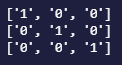
\includegraphics[width=4cm]{Images/Testing/T2.6.1.PNG} \\
    \vspace{1cm}

    {\large Evidence 2.\rn } \\ 
    \vspace{0.3cm}
    Matrix Addition Calculation \\
    \begin{pythoncode}
values = [[4, 3],
        [2, 1]]
matrix = Matrix(values)
values2 = [[3, 4],
    [1, 2]]
matrix2 = Matrix(values2)

result = matrix + matrix2
print(result)
    \end{pythoncode}
    The output of the above code: \\
    
\includegraphics[width=3cm]{Images/Testing/T2.7.1.PNG} \\
    \vspace{1cm}

    {\large Evidence 2.\rn } \\ 
    \vspace{0.3cm}
    Matrix Subtraction Calculation \\
    \begin{pythoncode}
values = [[4, 3],
        [2, 1]]
matrix = Matrix(values)
values2 = [[3, 4],
    [1, 2]]
matrix2 = Matrix(values2)

result = matrix - matrix2
print(result)  
    \end{pythoncode}
    The output of the above code: \\
    
\includegraphics[width=3cm]{Images/Testing/T2.8.1.PNG} \\
    \vspace{1cm}

    {\large Evidence 2.\rn } \\ 
    \vspace{0.3cm}
    Matrix Multiplication Calculation \\
    \begin{pythoncode}
values = [[4, 3],
        [2, 1]]
matrix = Matrix(values)
values2 = [[3, 4],
        [1, 2]]
matrix2 = Matrix(values2)

result = matrix * matrix2
print(result)
    \end{pythoncode}
    The output of the above code: \\
    
\includegraphics[width=3cm]{Images/Testing/T2.9.1.PNG} \\
    \vspace{1cm}

    {\large Evidence 2.\rn } \\ 
    \vspace{0.3cm}
    Matrix Scalar Multiplication Calculation \\
    \begin{pythoncode}
values = [[4, 3],
        [2, 1]]
matrix = Matrix(values)

result = matrix * 3 
print(result)
    \end{pythoncode}
    The output of the above code: \\
    
\includegraphics[width=3cm]{Images/Testing/T2.10.1.PNG} \\
    \vspace{1cm}

    {\large Evidence 2.\rn } \\ 
    \vspace{0.3cm}
    Vector Hadamard Product Calculation \\
    \begin{pythoncode}
values = [1, 2, 3, 4]
vector = Matrix(values)

values = [4, 3, 2, 1]
vector2 = Matrix(values)

result = vector * vector2
print(result)
    \end{pythoncode}
    The output of the above code: \\
    
\includegraphics[width=1.5cm]{Images/Testing/T2.11.1.PNG} \\
    \vspace{1cm}

    {\large Evidence 2.\rn } \\ 
    \vspace{0.3cm}
    Matrix Power Calculation \\
    \begin{pythoncode}
values = [[4, 3],
        [2, 1]]
matrix = Matrix(values)

result = matrix ** 5
print(result)
    \end{pythoncode}
    The output of the above code: \\
    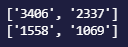
\includegraphics[width=3cm]{Images/Testing/T2.12.1.PNG} \\
    \vspace{1cm}

    {\large Evidence 2.\rn } \\ 
    \vspace{0.3cm}
    Matrix Transpose Calculation \\
    \begin{pythoncode}
values = [[4, 3],
        [2, 1]]
matrix = Matrix(values)

result = matrix.Transpose()
print(result)

    \end{pythoncode}
    The output of the above code: \\
    
\includegraphics[width=3cm]{Images/Testing/T2.13.1.PNG} \\
    \vspace{1cm}

    {\large Evidence 2.\rn } \\ 
    \vspace{0.3cm}
    Matrix Select Column \\
    \begin{pythoncode}
values = [[4, 3, 6],
        [2, 1, 5]]
matrix = Matrix(values)

result = matrix.SelectColumn(1)
print(result)
    \end{pythoncode}
    The output of the above code: \\
    
\includegraphics[width=1.5cm]{Images/Testing/T2.14.1.PNG} \\
    \vspace{1cm}

    {\large Evidence 2.\rn } \\ 
    \vspace{0.3cm}
    Matrix Select Row \\
    \begin{pythoncode}
values = [[4, 3, 6],
        [2, 1, 5]]
matrix = Matrix(values)

result = matrix.SelectRow(0)
print(result)
    \end{pythoncode}
    The output of the above code: \\
    
\includegraphics[width=3cm]{Images/Testing/T2.15.1.PNG} \\
    \vspace{1cm}
    
    {\large Evidence 2.\rn } \\ 
    \vspace{0.3cm}
    Vector Max \\
    \begin{pythoncode}
values = [4, 3, 6, 1, 2, 5]
vector = Matrix(values)

result = vector.MaxInVector()
print(result)
    \end{pythoncode}
    The output of the above code: \\
    
\includegraphics[width=1.5cm]{Images/Testing/T2.16.1.PNG} \\
    \vspace{1cm}
    
    {\large Evidence 2.\rn } \\ 
    \vspace{0.3cm}
    Matrix Clear \\
    \begin{pythoncode}
values = [[4, 3, 6],
        [2, 1, 5]]
matrix = Matrix(values)

matrix.Clear()
print(matrix)
    \end{pythoncode}
    The output of the above code: \\
    
\includegraphics[width=4cm]{Images/Testing/T2.17.1.PNG} \\
    \vspace{1cm}
    
    {\large Evidence 2.\rn } \\ 
    \vspace{0.3cm}
    Matrix Combine Vectors \\
    \begin{pythoncode}
values = [1, 2, 3, 4]
vector = Matrix(values)

values = [4, 3, 2, 1]
vector2 = Matrix(values)

vectorList = [vector, vector2]

result = Matrix.CombineVectorsHor(vectorList)
print(result)
    \end{pythoncode}
    The output of the above code: \\
    \includegraphics[width=3cm]{Images/Testing/T2.18.1.PNG} \\
    \vspace{1cm}
    
    {\large Evidence 2.\rn } \\ 
    \vspace{0.3cm}
    Matrix Sum \\
    \begin{pythoncode}
values = [[4, 3, 6],
        [2, 1, 5]]
matrix = Matrix(values)

result = matrix.Sum()
print(result)
    \end{pythoncode}
    The output of the above code: \\
    \includegraphics[width=1.5cm]{Images/Testing/T2.19.1.PNG} \\
    \vspace{1cm}
    
    {\large Evidence 2.\rn } \\ 
    \vspace{0.3cm}
    Console Output, all Tests have passed with no failures \\
    \includegraphics[width=6cm]{Images/Testing/T2.20.1.PNG} \\
    \vspace{1cm}

    {\large Evidence 2.\rn } \\ 
    \vspace{0.3cm}
    Console Output, all Tests have passed with no failures \\
    \includegraphics[width=6cm]{Images/Testing/T2.21.1.PNG} \\
    \vspace{1cm}

    {\large Evidence 2.\rn } \\ 
    \vspace{0.3cm}
    Console Output, all Tests have passed with no failures \\
    \includegraphics[width=6cm]{Images/Testing/T2.22.1.PNG} \\
    \vspace{1cm}

    {\large Evidence 2.\rn } \\ 
    \vspace{0.3cm}
    Console Output, all Tests have passed with no failures \\
    \includegraphics[width=6cm]{Images/Testing/T2.23.1.PNG} \\
    \vspace{1cm}
\end{center}

\subsubsection{Deep Q Learning Algorithm Evidence}

\setcounter{magicrownumbers}{0}
\begin{center}
    {\large Evidence 3.\rn } \\ 
    \vspace{0.3cm}
    The Neural Network objects in Memory
    \includegraphics{Images/Testing/T3.1.1.PNG}
    \vspace{1cm}
    
    {\large Evidence 3.\rn } \\ 
    \vspace{0.3cm}
    The layer sizes upon creating the Networks \\
    \includegraphics{Images/Testing/T3.2.1.PNG} \\
    The list of layer sizes in the parameters file \\
    \includegraphics{Images/Testing/T3.2.2.PNG}
    \vspace{1cm}

    {\large Evidence 3.\rn } \\ 
    \vspace{0.3cm}
    Actions being printed to console, predicted by the Network \\
    \includegraphics{Images/Testing/T3.3.1.PNG}
    \vspace{1cm}

    {\large Evidence 3.\rn } \\ 
    \vspace{0.3cm}
    Loss Vector printed to console \\
    \includegraphics{Images/Testing/T3.9.2.PNG}
    \vspace{1cm}

    {\large Evidence 3.\rn } \\ 
    \vspace{0.3cm}
    Average Loss Per Step negatively declines meaning the Back Propagation is Functional \\
    \includegraphics[width=12cm]{Images/Evaluation/RedWaterStaticExtra.png}
    \vspace{1cm}
    

    {\large Evidence 3.\rn } \\ 
    \vspace{0.3cm}
    Pushing items to the front of the Double Ended Queue \\

    \begin{pythoncode}
deque = Deque(10)
deque.PushFront(3)
print("Added 3:", deque.queue)
deque.PushFront(-5)
print("Added -1:", deque.queue)
deque.PushFront(9)
print("Added 9:", deque.queue)
    \end{pythoncode}
    
    The output of the above code: \\
    \includegraphics{Images/Testing/T3.8.1.PNG}
    \vspace{1cm}

    {\large Evidence 3.\rn } \\ 
    \vspace{0.3cm}
    Creating a Double Ended Queue with a length of 4, add Push Items to it, and get the 
    Items in First and Last \\

    \begin{pythoncode}
deque = Deque(4)
deque.PushFront(3)
deque.PushFront(-5)
deque.PushFront(9)
deque.PushFront(4)
deque.PushFront(-4)

print("First:", deque.First())
print("Last:", deque.Last())
print("Queue:", deque.queue)
    \end{pythoncode}

    The output of the above code: \\
    \includegraphics{Images/Testing/T3.9.1.PNG}
    \vspace{1cm}

    {\large Evidence 3.\rn } \\ 
    \vspace{0.3cm}
    Create a Double Ended Queue and Sample items from the Queue \\

    \begin{pythoncode}
deque = Deque(4)
deque.PushFront(3)
deque.PushFront(-5)
deque.PushFront(9)
deque.PushFront(4)
deque.PushFront(-4)

print("Sample 1:", deque.Sample(2))
print("Sample 2:", deque.Sample(2))
print(deque.queue)
    \end{pythoncode}

    The output of the above code: \\
    \includegraphics{Images/Testing/T3.10.1.PNG}
    \vspace{1cm}

    {\large Evidence 3.\rn } \\ 
    \vspace{0.3cm}
    Experience Replay buffer being sampled every 100 Steps \\
    \includegraphics{Images/Testing/T3.9.3.PNG} \\
    The parameters in Parameters file \\
    \includegraphics{Images/Testing/T3.9.4.PNG}
    \vspace{1cm}

    {\large Evidence 3.\rn } \\ 
    \vspace{0.3cm}
    Testing the Implemented Activations with specific values \\
    
    \begin{pythoncode}
outputVector = Matrix([-1, 0, 1])

Sigmoid = Sigmoid()
print("Sigmoid:")
print(Sigmoid.Activation(outputVector))

TanH = TanH()
print("TanH:")
print(TanH.Activation(outputVector))

ReLu = ReLu()
print("ReLu:")
print(ReLu.Activation(outputVector)) 

LeakyReLu = LeakyReLu()
print("LeakyReLu:")
print(LeakyReLu.Activation(outputVector))
    \end{pythoncode}

    The output of the above code: \\
    \includegraphics[width=3cm]{Images/Testing/T3.All.PNG} \\

    The WolframAlpha Sigmoid Results: \\
    \begin{figure}[H]
        \centering
        \subfloat{\includegraphics[width=4cm]{Images/Testing/T3Sigmoid-1.PNG}}
        \qquad
        \subfloat{\includegraphics[width=3cm]{Images/Testing/T3Sigmoid0.PNG}}
        \qquad
        \subfloat{\includegraphics[width=2.7cm]{Images/Testing/T3Sigmoid1.PNG}}
    \end{figure}
    

    The WolframAlpha TanH Results: \\
    \begin{figure}[H]
        \centering
        \subfloat{\includegraphics[width=3.2cm]{Images/Testing/T3Tanh-1.PNG}}
        \qquad
        \subfloat{\includegraphics[width=3cm]{Images/Testing/T3Tanh0.PNG}}
        \qquad
        \subfloat{\includegraphics[width=3.8cm]{Images/Testing/T3Tanh1.PNG}}
    \end{figure}

    The WolframAlpha ReLu Results: \\
    \begin{figure}[H]
        \centering
        \subfloat{\includegraphics[width=3.3cm]{Images/Testing/T3Relu-1.PNG}}
        \qquad
        \subfloat{\includegraphics[width=3cm]{Images/Testing/T3Relu0.PNG}}
        \qquad
        \subfloat{\includegraphics[width=2.7cm]{Images/Testing/T3Relu1.PNG}}
    \end{figure}

    The Leaky ReLu Results (Not supported by WolframAlpha): \\
    \begin{eqnarray*}
        \text{LeakyReLu}(x) &=&  \begin{cases}
            x < 0 & 0.1 \times x \\
            x >= 0 & x
        \end{cases} \\
        \text{LeakyReLu}(-1) &=& -1 \times 0.1 = -0.1 \\
        \text{LeakyReLu}(0) &=& 1(0) = 0 \\
        \text{LeakyReLu}(1) &=& 1(1) = 1 \\
    \end{eqnarray*}

    {\large Evidence 3.\rn } \\ 
    \vspace{0.3cm}
    Testing the Implemented Activation Derivatives with specific values \\
    
    \begin{pythoncode}
outputVector = Matrix([-1, 0, 1])

Sigmoid = Sigmoid()
print("Sigmoid Derivative:")
print(Sigmoid.Derivative(outputVector))

TanH = TanH()
print("TanH Derivative:")
print(TanH.Derivative(outputVector))

ReLu = ReLu()
print("ReLu Derivative:")
print(ReLu.Derivative(outputVector)) 

LeakyReLu = LeakyReLu()
print("LeakyReLu Derivative:")
print(LeakyReLu.Derivative(outputVector))
    \end{pythoncode}

    The output of the above code: \\
    \includegraphics[width=3cm]{Images/Testing/T3AllDer.PNG} \\

    The WolframAlpha Sigmoid Derivative Results: \\
    \begin{figure}[H]
        \centering
        \subfloat{\includegraphics[width=4cm]{Images/Testing/T3SigmoidDer-1.PNG}}
        \qquad
        \subfloat{\includegraphics[width=4.5cm]{Images/Testing/T3SigmoidDer0.PNG}}
        \qquad
        \subfloat{\includegraphics[width=3.5cm]{Images/Testing/T3SigmoidDer1.PNG}}
    \end{figure}

    The WolframAlpha TanH Derivative Results: \\
    \begin{figure}[H]
        \centering
        \subfloat{\includegraphics[width=3.2cm]{Images/Testing/T3TanhDer-1.PNG}}
        \qquad
        \subfloat{\includegraphics[width=3cm]{Images/Testing/T3TanhDer0.PNG}}
        \qquad
        \subfloat{\includegraphics[width=3.5cm]{Images/Testing/T3TanhDer1.PNG}}
    \end{figure}

    The ReLu Derivative Results (Not supported by WolframAlpha): \\
    \begin{eqnarray*}
        \text{ReLu}'(x) &=&  \begin{cases}
            x < 0 & 0 \\
            x >= 0 & 1
        \end{cases} \\
        \text{ReLu}'(-1) &=& 0 \\
        \text{ReLu}'(0) &=&  0 \\
        \text{ReLu}'(1) &=&  1 \\
    \end{eqnarray*}

    The Leaky ReLu Results (Not supported by WolframAlpha): \\
    \begin{eqnarray*}
        \text{LeakyReLu}'(x) &=&  \begin{cases}
            x < 0 & 0.1 \\
            x >= 0 & 1
        \end{cases} \\
        \text{LeakyReLu}'(-1) &=& 0.1 \\
        \text{LeakyReLu}'(0) &=& 0 \\
        \text{LeakyReLu}'(1) &=& 1 \\
    \end{eqnarray*}


\end{center}

\subsubsection{Data Logger Evidence}

\setcounter{magicrownumbers}{0}
\begin{center}
    {\large Evidence 4.\rn } \\ 
    \vspace{0.3cm}
    Randomnly Generated Unsorted List, sorted by the 1st Element to form the Sorted List \\

    \begin{pythoncode}
inputList = [[random.randint(-10,10), random.randint(-10,10)] for i in range(5)]
print("Unsorted List:")
for item in inputList:
print(item)

dl = DataCollector("SortingTest", [int, int], False)

dl.LogDataPointBatch(inputList)

sortedList = dl.HeapSort(0)

print("Sorted List:")
for item in sortedList:
print(item)
    \end{pythoncode}

    The output of the above code: \\
    \includegraphics[width=3cm]{Images/Testing/T4.1.1.PNG} \\

    \vspace{1cm}

    {\large Evidence 4.\rn } \\ 
    \vspace{0.3cm}
    Adding a single point: [5, 2] to DataLogger \\
    \begin{pythoncode}
dl = DataCollector("AddPointTest", [int, int], False)
print("Before: ", dl.dataPoints)

dl.LogDataPoint([5, 2])

print("After: ", dl.dataPoints)
    \end{pythoncode}

    The output of the above code: \\
    \includegraphics[width=4cm]{Images/Testing/T4.2.1.PNG} \\
    \vspace{1cm}

    {\large Evidence 4.\rn } \\ 
    \vspace{0.3cm}
    Test Data Point matches struture \\

    \begin{pythoncode}
dl = DataCollector("Match Single Types", [int, float], False)

print("Matches Structure: ", dl.CheckMatchStructure([-3, 2.2]))
    \end{pythoncode}

    The output of the above code: \\
    \includegraphics[width=4cm]{Images/Testing/T4.3.1.PNG} \\
    \vspace{1cm}

    {\large Evidence 4.\rn } \\ 
    \vspace{0.3cm}
    Test Data Point matches structure \\

    \begin{pythoncode}
dl = DataCollector("Match Multi Typed", [bool, [float, int]], False)

print("Matches Structure: ", dl.CheckMatchStructure([False, 4.5]))
print("Matches Structure: ", dl.CheckMatchStructure([True, -9]))
    \end{pythoncode}
        
    The output of the above code: \\
    \includegraphics[width=4cm]{Images/Testing/T4.4.1.PNG} \\
    \vspace{1cm}

    {\large Evidence 4.\rn } \\ 
    \vspace{0.3cm}
    Test Data Point matches structure \\

    \begin{pythoncode}
dl = DataCollector("Match List Type", [bool, str], False)

print("Matches Structure: ", dl.CheckMatchStructure([True, ["Matt", "Isabel", "Tristan", "Chris"]]))
    \end{pythoncode}
                    
    The output of the above code: \\
    \includegraphics[width=4cm]{Images/Testing/T4.5.1.PNG} \\
    \vspace{1cm}

    {\large Evidence 4.\rn } \\ 
    \vspace{0.3cm}
    Test error thrown when Data Point doesnt match the given structure \\

    \begin{pythoncode}
try:
dl = DataCollector("Match Data Structure Error", [str, int], False)

print("Matches Structure: ", dl.CheckMatchStructure(["Steve Preston", True]))
except Exception as x:
print(x)
    \end{pythoncode}

    The output of the above code: \\
    \includegraphics[width=8cm]{Images/Testing/T4.6.1.PNG} \\
    \vspace{1cm}

    {\large Evidence 4.\rn } \\ 
    \vspace{0.3cm}
    Select Prime numbers in 1st index\\

    \begin{pythoncode}
inputList = [[random.randint(-10,10), random.randint(-10,10)] for i in range(5)]
print("Random List:")
for item in inputList:
print(item)

dl = DataCollector("Select List", [int, int], False)

dl.LogDataPointBatch(inputList)

sortedList = dl.Select(0, [1,2,3,5,7])

print("Selected List:")
for item in sortedList:
print(item)
    \end{pythoncode}
        
    The output of the above code: \\
    \includegraphics[width=3cm]{Images/Testing/T4.7.1.PNG} \\
    \vspace{1cm}

    {\large Evidence 4.\rn } \\ 
    \vspace{0.3cm}

    Test for saving a file \\
    \begin{pythoncode}
inputList = [[random.randint(-10,10), random.randint(-10,10)] for i in range(5)]
print("Saved List:")
for item in inputList:
print(item)

dl = DataCollector("Save-Load Test", [int, int], False)

dl.LogDataPointBatch(inputList)

dl.SaveDataPoints()
    \end{pythoncode}

    The saved Data Points \\
    \includegraphics[width=3cm]{Images/Testing/T4.8.1.PNG} \\
    The saved file "Save-Load Test.data" \\
    \includegraphics[width=4cm]{Images/Testing/T4.8.2.PNG} \\
    \vspace{1cm}

    {\large Evidence 4.\rn } \\ 
    \vspace{0.3cm}

    Test for loading a file
    \begin{pythoncode}
dl = DataCollector("Save-Load Test", [int, int], True)

print("Loaded List:")
for item in dl.dataPoints:
print(item)
    \end{pythoncode}

    The File we're loading from "Save-Load Test.data" \\
    \includegraphics[width=4cm]{Images/Testing/T4.8.2.PNG} \\
    The loaded Data Points \\
    \includegraphics[width=3cm]{Images/Testing/T4.9.1.PNG} \\
    \vspace{1cm}
\end{center}

\subsubsection{Simulation Evidence}

\setcounter{magicrownumbers}{0}
\begin{center}
    {\large Evidence 5.\rn } \\ 
    \vspace{0.3cm}
    The Agent Object stored in Memory \\
    \includegraphics[width=9cm]{Images/Testing/T5.1.1.PNG} \\
    \vspace{1cm}

    {\large Evidence 5.\rn } \\ 
    \vspace{0.3cm}
    The Enemy Objects stored in Memory \\
    \includegraphics[width=9cm]{Images/Testing/T5.2.1.PNG} \\
    \vspace{1cm}

    {\large Evidence 5.\rn } \\ 
    \vspace{0.3cm}
    Video Evidence
    \vspace{1cm}

    {\large Evidence 5.\rn } \\ 
    \vspace{0.3cm}
    Tile Data Objects are returned in a Vector \\
    \includegraphics[width=6cm]{Images/Testing/T5.4.1.PNG} \\
    \vspace{1cm}

    {\large Evidence 5.\rn } \\ 
    \vspace{0.3cm}
    Grayscale Values in a Vector \\
    \includegraphics[width=4cm]{Images/Testing/T5.5.1.PNG} \\
    \vspace{1cm}

    {\large Evidence 5.\rn } \\ 
    \vspace{0.3cm}
    Reward on Left, and the chosen action on Right \\
    \includegraphics[width=2cm]{Images/Testing/T5.6.1.PNG} \\
    \vspace{1cm}

    {\large Evidence 5.\rn } \\ 
    \vspace{0.3cm}
    World Generated, is of an Acceptable Standard \\
    \includegraphics[width=8cm]{Images/Testing/T5.7.1.PNG} \\
    \vspace{1cm}

    {\large Evidence 5.\rn } \\ 
    \vspace{0.3cm}
    Changed Water Value creates no Water and more Beach \\
    \includegraphics[width=8cm]{Images/Testing/T5.8.1.PNG} \\
    \vspace{1cm}

    {\large Evidence 5.\rn } \\ 
    \vspace{0.3cm}
    Generated with seed 420 \\
    \includegraphics[width=8cm]{Images/Testing/T5.9.1.PNG} \\
    Generated again with the seed 420. Note different Trees, Enemy and Agent Positions, due to them not being
    tied to the Terrain Seed. \\
    \includegraphics[width=8cm]{Images/Testing/T5.9.2.PNG} \\
    \vspace{1cm}
    
\end{center}

\begin{flushleft}
    \huge
    \section{Evaluation}
    \vspace{0.1cm}

    \large
    \subsection{Evaluation of Objectives}
        \vspace{0.2cm}
        In this section, I will evaluate all of my objectives I set out to complete.
        \vspace{0.2cm}

        \subsubsection{Reading user inputted data}
            \vspace{0.2cm}
            The user can input the parameters through a json file, and these parameters are checked against a range file to check they are within
            the specified size. All of the parameters are read correctly and utilised within the Program. \\
            \vspace{0.2cm}
            The Machine Learning Data is read from .dqn files. The Learning is resumed from where it was saved from with all the Weights and
            Biases intact. \\

            \vspace{0.5cm}    
        \subsubsection{Generating the Environment}
            \vspace{0.2cm}
            At the start of the program an instance of World Class is created and the Generate methods are invoked. These methods utilise Perlin
            Noise and Poisson Disc Sampling. The Terrain values are stored in a 2d list of Tile Objects which store the Height, Type and Colour data
            for each Tile. The Poisson Disc Sampling Generates a list of points which Trees are then generated at those positions. The Width
            of the world and Tile colours are determined by the Input Parameters. \\

            \vspace{0.5cm}    
        \subsubsection{Displaying the world to a Pygame Window}
            \vspace{0.2cm}
            Upon generating the Map Data the Terrain is displayed in a grid to the Pygame Window, it is represented as a grid of tiles of the pixel 
            width loaded in by the Inputted Parameters. The Agent and Enemies are Drawn at their according positions, taking up entire Tile. If Debug
            mode is enabled, a representation of the Neural Network will be displayed on the right hand side of the window. \\

            \vspace{0.5cm}   
        \subsubsection{Simple Agent with a set of Actions}
            \vspace{0.2cm}
            An Agent can be created as an object and works along side the Dual Neural Network Object to enable interactions between the environment and
            the Network. The Agent can collect the surroundng Tile Data using the \textbf{GetTileVector} Method, this can then be converted into the
            Networks Input Vector using the \textbf{TileVectorPostProcess} Method. There exists Methods to Take a given Action, normally outputted by
            the Network. Along with Methods to Calculate Reward for an Action given a State, or the Maximum Possible Reward Given a State. \\
            \vspace{0.2cm}
            There also exists Methods to Reset the Agent to its default values. Along with Determining the Agents Spawn Position when given a WorldMap
            Object. \\

            \vspace{0.5cm}   
        \subsubsection{Matrix Class with Standard Operations}
            \vspace{0.2cm}
            A Matrix can be created using 3 different methods. First using a Tuple of Integers, a new Matrix will be created of that size, with initialised
            0 values. Second using a prexisting 2d list of values, a new Matrix will be created with these dimensions and values. Thirdly a 1d list of
            values can be used to create a 1 wide Vector of values, where it reads each value into the 1st position of each row. \\
            \vspace{0.2cm}
            All standard operations for the Matrix Object are implemented using Operator Overloading to make code less bloated. All are written 
            efficiently utilising minimum complexity algorithms. Addition can be carried out utilising the $+$ Operator. Subtraction can be carried out
            utilising the $-$ Operator. Multiplication and Scalar Multiplication are both carried out utilising the $*$ Operator. Power Operation is
            carried out utilising the $\string^$ operator. A Matrix can be converted to a Formatted String implicitly by using it in a string context. \\
            \vspace{0.2cm}
            All Matrice Operations have appropriate Exceptions with descriptive Error Messages. They will throw errors when incorrect Data is provided to
            the specified Operation. \\

            \vspace{0.5cm}   
        \subsubsection{Creation of a Reinforcement Learning Model}
            \vspace{0.2cm}
            A Dual Neural Network can be created as an object, which stores two Neural Network Objects, Main and Target. The Dual Neural Network
            contains the Primary Method \textbf{Step} which invokes a Series of Lower Level Methods to perform a singular Time Step. The Neural 
            Network Object store a List of Layers Objects which are dynamically created from the Input Parameters. Each Layer contains a Weight 
            Matrix, Bias Vector, and Output Vector. The Lowest Level methods for Forward and Back Propagation are contained within the Layer Object. \\
            \vspace{0.2cm}
            First Forward Propagation occurs on the Main and Target Network. Then results of the Main Network are taken to choose the action for the Agent. 
            Epsilon Greedy is implemented to determine whether to choose the random or predicted result. This Action is then fed to the Agent, along with 
            calculating the reward for that Action. The Loss of the Main Network is then calculated using a modified Bellman Equation for Dual Neural 
            Networks. This Loss is used for Back Propagating the Main Neural Network. The Main Networks Weights are copied to the Target Network
            every specified ammount of steps. Every specified ammount of steps, Experience Replay is performed to learn from past experiences again. \\
            \vspace{0.2cm}
            The combination of these steps form a functional Dual Neural Network utilising a Reinforcement Learning Model. \\

            \vspace{0.5cm}   
        \subsubsection{Creation of a Data Logger}
            \vspace{0.2cm}
            A Data Logger Class can be used to Log and Store Data Points at various parts of the Program. Each Data Point is stored as a Tuple of Values
            as part of a .data file. These files are stored as Binary Files, and are Read into the Program upon launch. \\
            \vspace{0.2cm}
            As part of the Data Logger you can sort points utilising a Heap Sort to sort through Data. \\

            \vspace{0.5cm}   

        \vspace{0.5cm}
    \subsection{Answering my Investigations Question}
        \vspace{0.2cm}
        As part of my Machine Learning Investigation I proposed the Question:

        \vspace{0.3cm}\begin{center}
        \textbf{Can you train a Machine Learning algorithm to survive in a pseudo random, open-world environment?}
        \end{center}\vspace{0.3cm}

        I aimed to answer this question by designing and creating a Deep Reinforcement Learning Model utilising a Deep Neural Network, along 
        with designing a Simple Simulation for a Machine Learning Agent to survive in. This simulation

        \vspace{0.5cm}

    \subsection{Expert Feedback}
        \vspace{0.2cm}
        I went back to my Expert Shaun in order to collect feedback on my finalised Technical Solution. I asked him a few Questions about my
        project, paraphrased where neccesary. \\
        \vspace{0.5cm}

        \begin{enumerate}
            \item What do you think of the Program? \\
                \vspace{0.2cm}
                "Overall I think your project is incredibly visually interesting to look at, I could stare at the graphical output for hours
                just rooting for the Agent to better itself and kill the Generated Enemies. The User Inputted Parameters are easy to change
                through the json file, and it is helpful that they are locked between certain ranges to stop the User from crashing their Pc
                from allocating too much memory. The Terrain generation looks pretty good for just a 4 coloured map generated from Perlin Noise.
                The Neural Network works as intended, although \textbf{NOT FINISHED}"

            \item Does my Tehnical Solution achieve all of the Set Goals and Objectives? \\
                \vspace{0.2cm}
                "The Program achieves all of the objectives you set out to complete, and it is clear alot of hard work went into completing your
                project. Lots of research needs to be carried out in order to understand the complexity behind Reinforcement Learning and all
                of its individual parts. Debugging this process also becomes increasingly difficult, due to the complex calculations, this 
                demonstrates you have the ability to solve problems independently. \\
                \vspace{0.2cm}
                You've also implemented an entire simulation ontop of the Dual Neural Network. Which uses even more complex algorithms, this demonstrates
                you can develop multiple Vertical Slices of a project, and intertwine them together in order to create one bigger project. This
                takes planning skill and a good understanding of OOP in order to pull off." \\

                \vspace{0.5cm}
            \item What Criticisms/Improvements would you suggest? \\
                \vspace{0.2cm}
                "Considering the scope of the project, youve carried out your completion of this task very well. The only suggestion I would have is
                to implement a Convolution, which might solve your Training Accuracy Problems. Otherwise a Description of your Project could be
                printed to console when the main file is run, or a 'Readme' text file included in the project files would useful to any users who 
                have little to no experience with Reinforcement Learning." \\

                \vspace{0.5cm}
        \end{enumerate}


        \vspace{0.5cm}
    \subsection{Evaluation of Expert Feedback}
        \vspace{0.2cm}
        

        \vspace{0.5cm}

    \subsection{System Improvements}
        \vspace{0.2cm}
        Overall I am happy with my Technical Solution. I achieved all the objectives I set out to complete in my Analyis. I have definitely achieved
        my primary goal of gaining a deeper understanding about the Maths and Logic behind how Neural Networks work. This has given me a Window into
        the field of Machine Learning and Artificial Intelligence, which I intend to pursue as part of my later Studies. \\
        \vspace{0.2cm}
        The Improvements I would like to make to my Technical Solution are: \\
        \vspace{0.5cm}

        \begin{enumerate}
            \item The Implementation of a Convolutional Neural Network was something I came across in my Initial Research and was mentioned by my Expert.
            Convolution carries out Pre-Processing on the inputted data before it is even touched by the Neural Network. This in theory would increase
            the training accuracy of my Network leading to better Results. \\
            
            \vspace{0.2cm}
            \item The Optimisation of my Matrix Class by compiling it into $C$ through the use of Cython would help speed up the training of the Neural
            Network. Due to Python being an interpretted language it is comparatively slow compared to the other programming languages I considered
            using. $C$ is a compiled language so it is comparatively alot faster, about 45 times faster according to some sources online. This could
            provide an easy way to optimise my Program without having to convert my entire Codebase into a different Language. \\

            \vspace{0.2cm}
            \item An increase in complexity of my simulation would provide a greater challenge towards my Agent and Neural Network. I could add a basic
            crafting system to convert the collected Wood into a sword, or a Hunger Bar so the Agent has to collect food and water in order to survive.
            I feel as though the Network wouldnt be able to solve these problems effectively though without the implementation of my first improvement,
            a Convolutional Neural Network. \\

            \vspace{0.2cm}
        \end{enumerate}
        \vspace{0.5cm}
\end{flushleft}

\begin{flushleft}
    \section{Technical Solution}
        This section includes all the code relating to my Technical Solution, along with the two Json Formatted files which
        are used within my project. 

        \begin{itemize}
            \item \hyperref[sec:main.py]{main.py - pg. \pageref{sec:main.py}}
            \item \hyperref[sec:simulation.py]{simulation.py - pg. \pageref{sec:simulation.py}}
            \item \hyperref[sec:newAgent.py]{newAgent.py - pg. \pageref{sec:newAgent.py}}
            \item \hyperref[sec:enemy.py]{enemy.py - pg. \pageref{sec:enemy.py}}
            \item \hyperref[sec:worldClass.py]{worldClass.py - pg. \pageref{sec:worldClass.py}}
            \item \hyperref[sec:perlinNoise.py]{perlinNoise.py - pg. \pageref{sec:perlinNoise.py}}
            \item \hyperref[sec:deepqlearning.py]{deepqlearning.py - pg. \pageref{sec:deepqlearning.py}}
            \item \hyperref[sec:matrix.py]{matrix.py - pg. \pageref{sec:matrix.py}}
            \item \hyperref[sec:activations.py]{activations.py - pg. \pageref{sec:activations.py}}
            \item \hyperref[sec:datalogger.py]{datalogger.py - pg. \pageref{sec:datalogger.py}}
            \item \hyperref[sec:heap.py]{heap.py - pg. \pageref{sec:heap.py}}
            \item \hyperref[sec:plotData.py]{plotData.py - pg. \pageref{sec:plotData.py}}
            \item \hyperref[sec:paramfile]{Parameters File - pg. \pageref{sec:paramfile}}
            \item \hyperref[sec:rangefile]{Range File - pg. \pageref{sec:rangefile}}
        \end{itemize}

        Key Algorithms and Data Structures within my Program can be Located as shown below.

        \begin{itemize}
            \item Matrix Implementation - Contained within matrix.py - pg. \pageref{sec:matrix.py}
            \item Deque Implementation - deepqlearning.py - pg.\pageref{sec:deepqlearning.py} - Line. 255
            \item Heap Implementation - Contained within heap.py - pg. \pageref{sec:heap.py}
            \item Heap Sort - datalogger.py - pg. \pageref{sec:datalogger.py} - Line. 68
            \item Experience Replay - deepqlearning.py - pg. \pageref{sec:deepqlearning.py} - Line. 129
            \item Forward Propagation - deepqlearning.py - pg. \pageref{sec:deepqlearning.py} - Line. 226
            \item Backwards Propagation - deepqlearning.py - pg. \pageref{sec:deepqlearning.py} - Line. 231
            \item Abstract Base Class Activation - Contained within activations.py - pg. \pageref{sec:activations.py}
            \item Perlin Noise Algorithm - Contained within perlinNoise.py - pg. \pageref{sec:perlinNoise.py}
            \item Poisson Disc Sampling - worldClass.py - pg. \pageref{sec:worldClass.py} - Line. 116
            \item Threaded Terrain Generation - worldClass.py - pg. \pageref{sec:worldClass.py} - Line. 55
            \item Checking Parameters - simulation.py - pg. \pageref{sec:simulation.py} - Line. 145
            \item Matching Data Point Structure - datalogger.py - pg. \pageref{sec:datalogger.py} - Line. 25
        \end{itemize}

        The Full Source Code is available publically through the Link Below. \\
        \vspace{0.5cm}
        \centerline{\textit{https://github.com/TheTacBanana/CompSciNEA}}

        \label{sec:main.py}
        \subsection{main.py}
        \inputminted[frame=leftline,framesep=2mm,baselinestretch=1.2,fontsize=\normalsize,linenos,breaklines]{python}{../Scripts/main.py}

        \label{sec:simulation.py}
        \subsection{simulation.py}
        \inputminted[frame=leftline,framesep=2mm,baselinestretch=1.2,fontsize=\normalsize,linenos,breaklines]{python}{../Scripts/simulation.py}

        \label{sec:newAgent.py}
        \subsection{newAgent.py}
        \inputminted[frame=leftline,framesep=2mm,baselinestretch=1.2,fontsize=\normalsize,linenos,breaklines]{python}{../Scripts/newAgent.py}

        \label{sec:enemy.py}
        \subsection{enemy.py}
        \inputminted[frame=leftline,framesep=2mm,baselinestretch=1.2,fontsize=\normalsize,linenos,breaklines]{python}{../Scripts/enemy.py}

        \label{sec:worldClass.py}
        \subsection{worldClass.py}
        \inputminted[frame=leftline,framesep=2mm,baselinestretch=1.2,fontsize=\normalsize,linenos,breaklines]{python}{../Scripts/worldClass.py}

        \label{sec:perlinNoise.py}
        \subsection{perlinNoise.py}
        \inputminted[frame=leftline,framesep=2mm,baselinestretch=1.2,fontsize=\normalsize,linenos,breaklines]{python}{../Scripts/perlinNoise.py}

        \label{sec:deepqlearning.py}
        \subsection{deepqlearning.py}
        \inputminted[frame=leftline,framesep=2mm,baselinestretch=1.2,fontsize=\normalsize,linenos,breaklines]{python}{../Scripts/deepqlearning.py}

        \label{sec:matrix.py}
        \subsection{matrix.py}
        \inputminted[frame=leftline,framesep=2mm,baselinestretch=1.2,fontsize=\normalsize,linenos,breaklines]{python}{../Scripts/matrix.py}

        \label{sec:activations.py}
        \subsection{activations.py}
        \inputminted[frame=leftline,framesep=2mm,baselinestretch=1.2,fontsize=\normalsize,linenos,breaklines]{python}{../Scripts/activations.py}

        \label{sec:datalogger.py}
        \subsection{datalogger.py}
        \inputminted[frame=leftline,framesep=2mm,baselinestretch=1.2,fontsize=\normalsize,linenos,breaklines]{python}{../Scripts/datalogger.py}

        \label{sec:heap.py}
        \subsection{heap.py}
        \inputminted[frame=leftline,framesep=2mm,baselinestretch=1.2,fontsize=\normalsize,linenos,breaklines]{python}{../Scripts/heap.py}

        \label{sec:plotData.py}
        \subsection{plotData.py}
        \inputminted[frame=leftline,framesep=2mm,baselinestretch=1.2,fontsize=\normalsize,linenos,breaklines]{python}{../Scripts/plotData.py}

        \label{sec:paramfile}
        \subsection{Parameters File}
        \inputminted[frame=leftline,framesep=2mm,baselinestretch=1.2,fontsize=\normalsize,linenos]{json}{../Parameters/Default.param}

        \label{sec:rangefile}
        \subsection{Ranges File}
        \inputminted[frame=leftline,framesep=2mm,baselinestretch=1.2,fontsize=\normalsize,linenos]{json}{../Parameters/Range.param}

\end{flushleft}

\end{document}